\chapter{Data Preparation and Processing}
\label{chapter:data_prep_and_proc}
The data volume of interferometric measurements inherently scale as the square of the number of antennas in the array ($N_{\rm ant}$). Not only does the sheer volume of data from large-$N_{\rm ant}$ arrays pose a problem for data storage, but also it requires precise and efficient efforts to quality assure (QA) the data. 

In this chapter, I will outline some of the efforts involved in data preparation, preprocessing and QA that are required for an EoR power spectrum estimate.

\section{Data Compression}
\label{sec:data_compression}

The PAPER-128 correlator produced 288 {\sc miriad} files per night. Each of these contained 8126 baselines, and each baseline contained visibilities over 1024 $98$\,kHz frequency channels and 56 $10$\,s time integrations. The four instrumental polarizations were in separate files. In sum, each file was 4.2 GB which meant that each night 1.2 TB of data were recorded.

In order to efficiently transport the data over Gigabit Ethernet from the Karoo Radio Quiet Zone (KRQZ) to Cape Town, and from Cape Town under transatlantic cables to Philadelphia, some compression was required. It was also required that such a compression, while lossy, did not effect the targeted cosmological signal.

\subsection{Delay--Delay-Rate Filtering}

The compression algorithm implemented for PAPER observations, Delay--Delay-Rate (DDR) filtering, was introduced in \cite{ParsonsBacker.09} described in \cite{Parsons.14}, and we briefly review it below.

The geometric delay of a celestial signal, originating form direction $\hat{s}$, incident on an interferometric baseline described by vector $\vec{b}$, is

\begin{equation}
\tau_g = |\vec{b} \cdot \hat{s}|/c
\end{equation}

where $c$ is the speed of light. This relationship implies that $\tau_g$ is bounded for a given baseline

\begin{equation}
- |\vec{b}|/c \leqslant \tau_g \leqslant |\vec{b}|/c
\label{eq:geometric_delay_bound}
\end{equation}

Equation~\ref{eq:geometric_delay_bound} therefore gives the maximum value of $|\tau_g|$ physically meaningful for a given array -- the maximum baseline length in that array, divided by $c$. For PAPER, the maximum baseline length is 300\,m, corresponding to $\max(|\tau_g|) = 1\mu$s. 
As reviewed in Chapter~\ref{chapter:eor_window_theory}, the delay axis may be accessed by Fourier transforming a visibility along the frequency axis. Once in delay space, power at delays larger in magnitude than $1 \mu$s could be removed. With a sufficiently large frequency bandwidth, this would not produce aliased signal, according to the critical Nyquist rate. By using the $1 \mu$s as a delay bound for all visibilities, the frequency axes of all compressed visibilities remained the same (reduced in number from 1024 to 203), which while sub-optimal from a compression point of view, allowed for ease of programming at later stages.

A similar geometric bound can be obtained by Fourier transforming the time axis of visibilities, provided that they were obtained in drift-scan mode (see Chapter~\ref{chapter:interferometry}). \cite{ParsonsBacker.09} showed that the rate at which the geometric delay on an interferometric baseline changes is governed only by the position of the array on Earth, and the Earth's rotation:

\begin{equation}
\dot{\tau}_g = -\frac{\omega_{\Earth} \cos\delta}{c} \left( b_x\sin\alpha + b_y\cos\alpha\right)
\end{equation}

where $\omega_{\Earth}$ is the angular frequency of the Earth's rotation, $\alpha$ and $\delta$ are the hour-angle and declination of a point on the celestial sphere, respectively, and $\vec{b}=(b_x,b_y,b_z)$ is the baseline vector expressed in equatorial coordinates.

For arrays not close to the geographic poles, $|b_y| \gg |b_x|$, there is a maximum rate of change (corresponding to ($\alpha$, $\delta$) = (0, 0)), producing a bound on $\dot{\tau}_g$:

\begin{equation}
- \omega_{\Earth}|b_y|/c \leqslant \dot{\tau}_g\leqslant \omega_{\Earth} |b_y|/c
\label{eq:geometric_delay_rate_bound}
\end{equation}

for a 300\,m East-West baseline, the maximum delay-rate is approximately $\max(|\dot{\tau}_g|) = 0.07$\,ns\,s$^{-1}$. This delay-rate was not Nyquist sampled by a single PAPER file: requiring the previous and next files generated for that polarization to be appended on either side of each visibility's time axis to prevent aliasing from the decimation. For the large scale processing of months of data, this required a software pipeline described in Section~\ref{subsec:compression_software}.

There are also other issues with DDR compression, largely associated with instrument systematics. Delay transforms rely on the fact that the bright foregrounds that dominate the measured signal are spectrally smooth, and that the frequency response of the instrument is also spectrally smooth: this of course is the basis for the EoR window paradigm reviewed in Chapter~\ref{chapter:eor_window_theory}. Likewise, delay-rate filtering assumes temporal smoothness. Radio Frequency Interference (RFI) signals created by human communications violate both models of smoothness, since they are typically confined to narrow bandwidths (creating sharp spikes along the frequency axis) and may be transient (creating sharp spikes along the time axis). This requires steadfast identification and flagging algorithms for RFI (see Section~\ref{sec:RFI}), and some variety of interpolation, fitting, or CLEANing across the flagged regions prior to compression.

By DDR filtering of PAPER-128 data using a 300\,m baseline to set the width of the filters we were able to reduce the volume of the data by an approximate factor of 70.

\subsection{Software Implementation}
\label{subsec:compression_software}

The first season of PAPER-128 data, due to a variety of circumstances, required compression on the computing cluster at the University of Pennsylvania. The raw data were stored on a high-volume drive that was able to connect with the cluster via a low-speed switch. The hardware capable of performing any sort of high-performance processing (i.e. holding the data in RAM) were ten `compute nodes' connected to the cluster via a high-speed switch, and mounted in an NFS architecture. The compute nodes could only hold $\sim 10$ PAPER-128 files in storage. 

The processing stages for compression of a night of PAPER data, described below, required knowledge of the location and compression state of not only individual files, but also the neighbors-in-time of the file in question, in order to implement the DDR filter described above. To supervise the compression we created a MySQL database, which we interacted with via Shell and Python scripts. The database contained a table for the data files under processing and their compression state, a table of neighbor-relations, a table of file details, and a table of the processing nodes available. The schema of this database is shown in Figure~\ref{fig:database_schema}.

\begin{figure}[h]
\centering
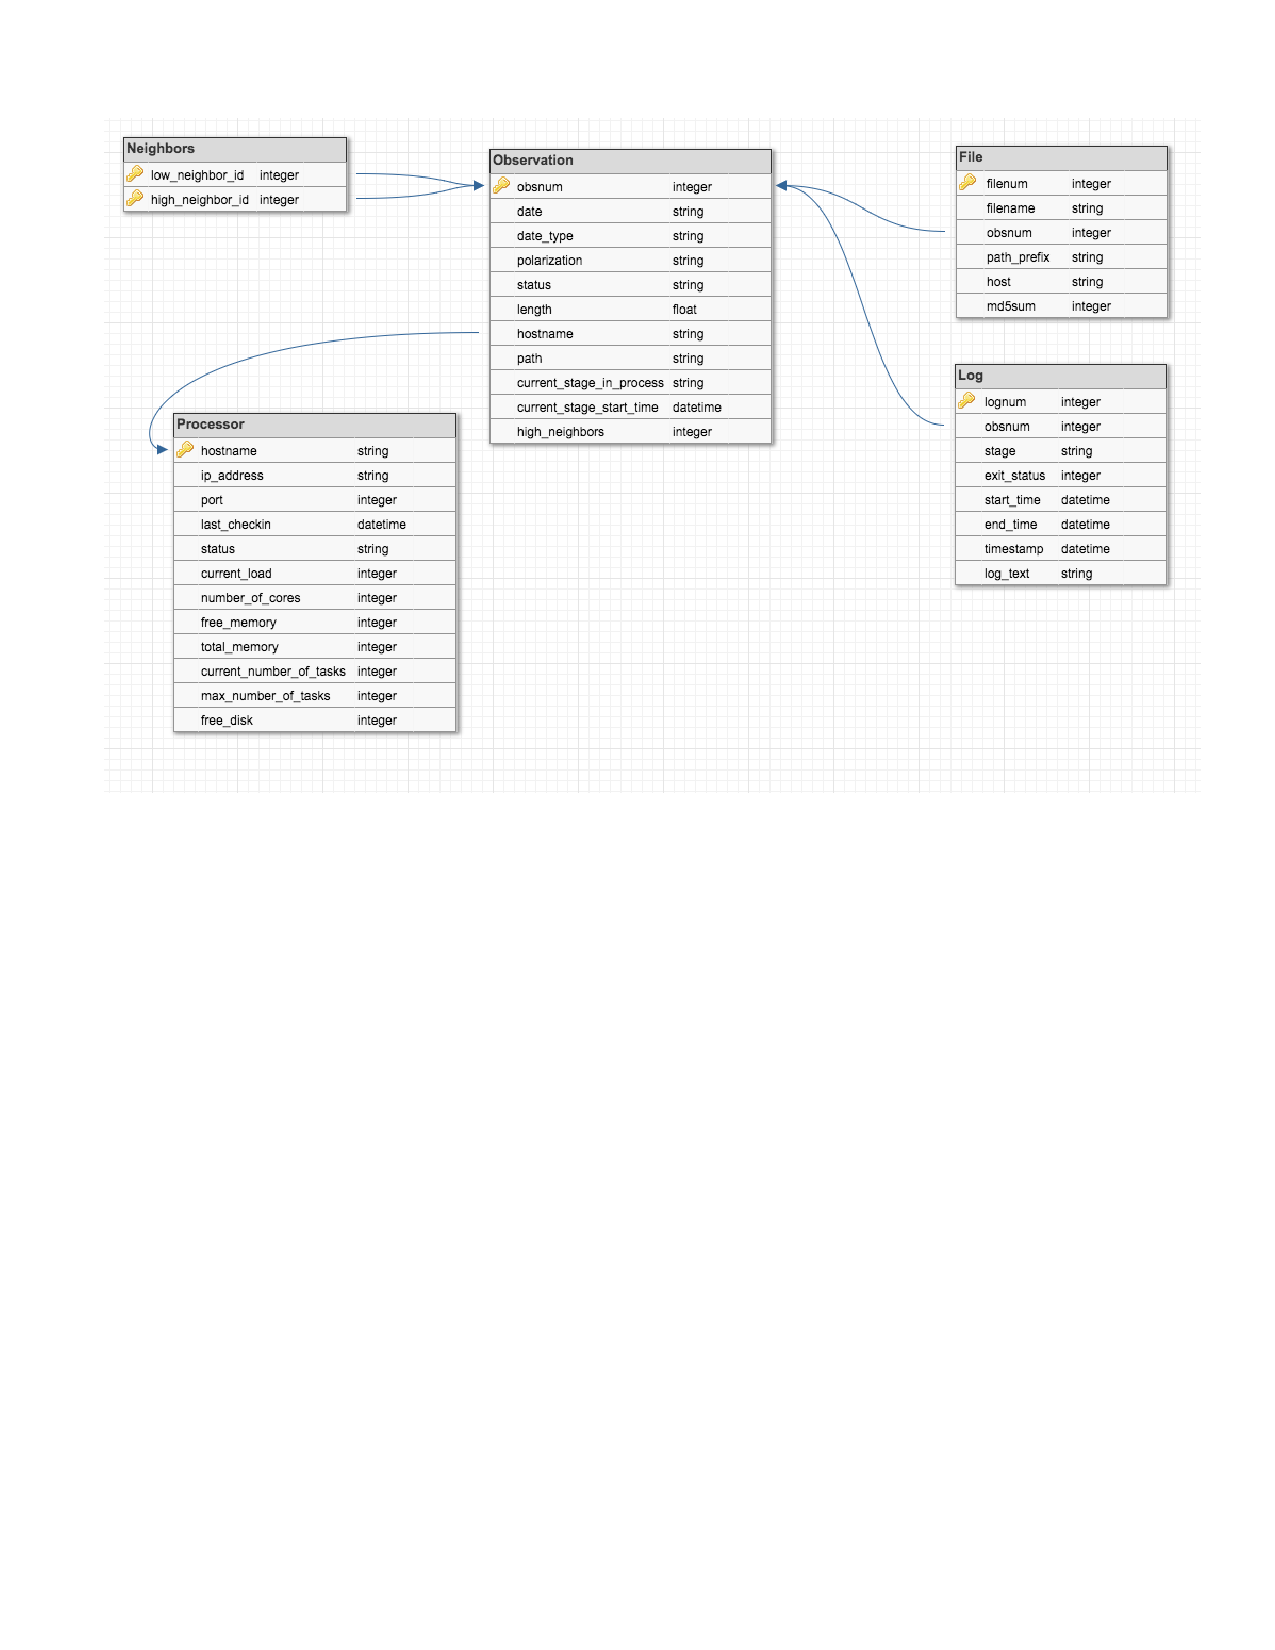
\includegraphics[scale=0.7]{chapters/data_processing/figures/RTP_diagram.pdf}
\caption[The schema of the database used to organize and implement PAPER data compression.]{The schema of the database used to organize and implement PAPER data compression.}
\label{fig:database_schema}
\end{figure}

To implement the compression, per file, the following steps were required:

\begin{enumerate}
\item Copying the file from the storage volume to the cluster. For a single night of data, this required roughly 8 hours.
\item Copying the file from the cluster to the compute node. This required roughly 5 minutes.
\item Generate copy of the file, with metadata corrections. This required roughly 1 minute.
\item Delete the raw file.
\item RFI-flag the high frequency-resolution data. This required roughly 2 minutes.
\item Delete the metadata-corrected file.
\item Acquire time-neighbors to the file in question, and bring them to the RFI-flagged stage. The time required for this stage varied with cluster activity, but usually required roughly 20 minutes.
\item DDR filter the RFI-flagged data, using an high-tolerance iterative CLEAN. This required roughly 20 minutes.
\item RFI flag the compressed data (coarse flagging), saving the flags to a separate file. This required roughly 1 minute.
\item Apply the coarse RFI flags to the \textit{uncompressed}, RFI-flagged data. This required roughly one minute.
\item DDR filter the now twice-RFI-flagged data, using a low-tolerance iterative CLEAN. This required roughly 120 minutes.
\item Copy compressed data to the cluster.
\item Delete the twice-RFI-flagged data.
\item If the once-RFI-flagged data are not required as neighbors, delete them.
\item Delete the compressed data from the compute node.
\item If neighbors have already been compressed, delete them, otherwise begin their compression.
\item After all files are compressed, delete the uncompressed files from the cluster.
\end{enumerate}

In total, this meant that across ten compute nodes, and efficient use of the fact that the neighbors could progress through the processing stages while the central file was being compressed, meant that it took roughly 20 to 24 hours to compress a night of observations. 

\section{Radio Frequency Interference}
\label{sec:RFI}

As noted above, RFI was able to introduce spectral and temporal structure that would cause ringing in the data during compression if it was not flagged. This meant that both identification and characterization of RFI was crucial to the scientific goals of the PAPER and HERA experiments. In Section~\ref{subsec:rfi_paper128}, I present characterization of RFI in the second season of PAPER-128 data. By averaging flags in local time I was able to investigate ``repeat offender'' frequency bands and identify outlying ``quiet'' and ``loud'' days.
In Section~\ref{subsec:rfi_hera19paper19} I analyze RFI flags from the first Internal Data Release (IDR1) of HERA commissioning data, which contained 19 HERA feeds suspended above 5\,m dishes in a close-packed hexagon, and 19 PAPER feeds in the same positions as the central dishes, allowing us to investigate the difference in flagging between feeds at different altitudes.

\subsection{PAPER-128}
\label{subsec:rfi_paper128}

The PAPER-128 2014 observation season ran from 18th June 2014 through the 30th April 2015. During this run, some 150 nights of data were recorded. A ``night'', which I will refer to using the JD at the start of observations, consists of twelve hours of observation from 6pm to 6am South African Standard Time (SAST). Observations as processed by the PAPER correlator are recorded in {\sc miriad} uv files. These files contain visibilities for each antenna pair in the array. Each integration is 20 seconds long over 1024 frequency bins from 100 to 200\,MHz. Each uv file contains 56 integrations per antenna pair, and 72 uv files are recorded per linear polarization (xx, xy, yx, yy) per night.

Early in the PAPER data compression process, visibilities are flagged for RFI. This is accomplished by the {\tt aipy} script \textit{xrfi\_simple.py}, which takes the derivative of the frequency axis of all baselines associated with a single antenna, and flags any frequencies with a derivative $\geqslant 6\sigma$ above the mean. We always flag the band-edges ($\sim$7\,MHz on each side), since these frequencies are not useful to us, and always flag the 137$\pm$0.6\,MHz band associated with ORBCOMM satellite network transmissions. This process is repeated per integration within each uv file and stored in a Python numpy zip (npz) file. This means that any baseline associated with antenna 1 can contribute a flag to the resultant npz file, which in turn is applied to the data.

The result is 280 files of high-time and -frequency resolution files per night per linear polarization containing information about the RFI environment of the HERA site. I report on the properties of these flags in time- and frequency-space over the 2014 observation season. This section is organized it as follows: in Section~\ref{subsubsec:avgprops}, I analyse the average properties of RFI over the season by stacking flags in local time and normalizing appropriately. In Section~\ref{subsubsec:indivprops} I address nights with particularly strange RFI properties. I discuss the implications of my findings in Section~\ref{subsubsec:rfi_paper128_conc}.

\subsubsection{Average Properties}
\label{subsubsec:avgprops}

In order to assess the average properties of the RFI environment, I calculated a weighted average of flags over the season. Over 150 nights, one-time occurrences are washed-out beneath the 1\% level, allowing me to assess persistent issues.

Nominally, each night should grant 3920 integrations-worth of flags over 1024 frequency bins, per linear polarization. In reality, most of the time this holds true, but occasionally not all files are compressible (hence failing to generate flags) or observations fail to start at the correct time (so there are no data to flag). Also, in the event of an X-engine failure within the correlator, contiguous chunks of the band (in eighths, i.e. 25\,MHz across) are flagged-out, usually for the rest of the night.

For this reason, I calculated a weighted average of the flags across the season, but neglected nights with correlator failures or late starts. Weights were simply the number of nights that contained that integration-bin in SAST. The resultant ``flag density waterfall'' is shown in Figure~\ref{fig:rfi_psa128_waterfall}. The color scale is indicative of flagging frequency across the season, and line plots above and to the right of the the waterfall showing the percentage of times and frequencies that were flagged, respectively. 

A summary of the persistent (flagged $\geq1\%$ of the time per channel) RFI frequencies can be found in Table~\ref{tab:rfi_psa128}. I have investigated each frequency and tried to find the most likely source for each. In most cases, this required looking at the properties in time as well as frequency. Others were more obvious from frequency alone, e.g. the 149.8\, MHz transmission frequency from the International Space Station (ISS). Still others I could not track down a convincing explanation for, and these are listed with a `?'. A `?' next to a possible cause indicates that the listed cause is the most prevalent at that frequency, but that the temporal properties of that cause do not necessarily make sense. Many of the characterizations arise from the South African Table of Frequency Allocations (SATFA; \cite{SAFreqTable}).

\begin{figure}[h!]
\centering
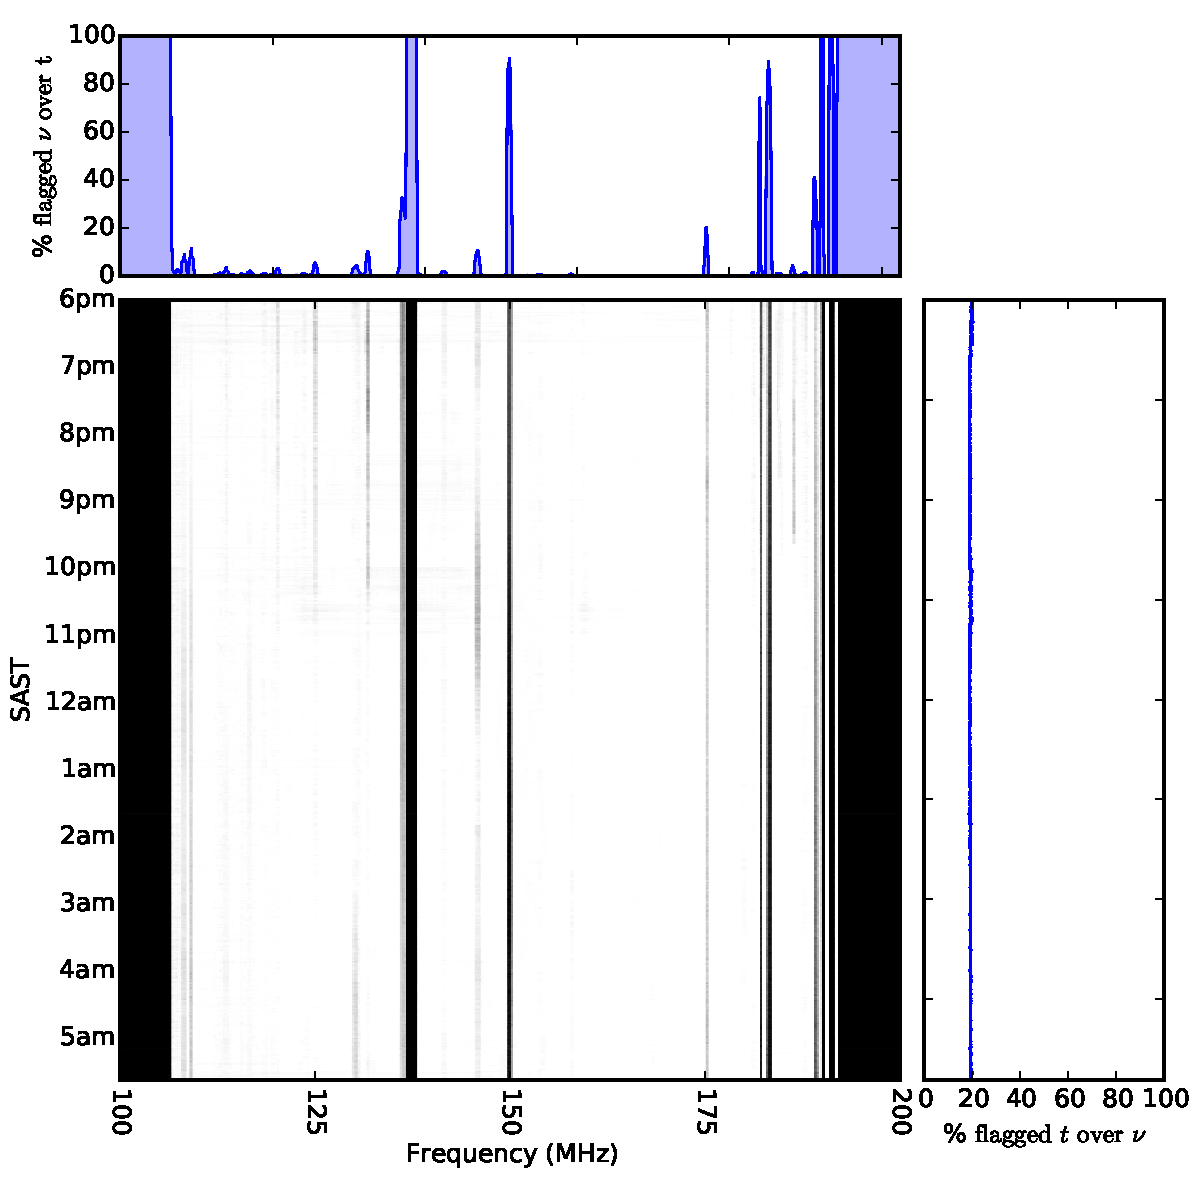
\includegraphics[width=\textwidth]{chapters/data_processing/figures/RFI_all_128.pdf}
\caption[A waterfall plot of RFI flags averaged over 150 days of PAPER-128 data.]{A waterfall plot of RFI flags averaged over 150 days of data. The gridding process is described in the text. Above the waterfall I show the percentage of the season each frequency is flagged, and to the right I show the percentage of frequencies that are flagged per integration.}
\label{fig:rfi_psa128_waterfall}
\end{figure}

\begin{deluxetable}{llll}
\centering
\label{tab:rfi_psa128}
\tablewidth{0pt}
\tablecaption{PAPER-128 RFI frequencies and brief characterization for the averaged flags.}
\tabletypesize{\footnotesize}
\tablehead{
\colhead{$\nu$} & \colhead{Flagged} & \colhead{Cause} & \colhead{Notes or} \\
\colhead{MHz} & \colhead{\%} & \colhead{(Possible)} & \colhead{Time (SAST) Characterization} \\
}
\startdata
103	$\pm$	3	&	100	&	BAND EDGE	&	Built-in to flagger.	\\
107.25	$\pm$	0.25	&	2.6	&	FM radio	&	Constant background at 2\% level	\\
107.55	$\pm$	0.05	&	1.9	&	FM radio	&	Constant background at 2\% level	\\
108.1	$\pm$	0.4	&	9	&	FM radio?	&	Rises with time, peaking at midnight and 4am	\\
109	$\pm$	0.4	&	11.5	&	FM radio?	&	Rises with time, peaking around 4am	\\
112.8	$\pm$	0.1	&	1.4	&	Aircraft?	&	Constant background at 1\% level	\\
114.05	$\pm$	0.85	&	3.7	&	?1	&	Decreases till midnight; peak at 4am	\\
116.55	$\pm$	0.35	&	2.2	&	?2	&	Peak at midnight	\\
120.15	$\pm$	0.35	&	3.2	&	Aircraft	&	Roughly follows CPT$\leftrightarrow$JNB flight times	\\
124.95	$\pm$	0.35	&	5.5	&	Aircraft	&	Roughly follows CPT$\leftrightarrow$JNB flight times	\\
130.25	$\pm$	0.55	&	4.3	&	?3	&	Falls (7pm) and rises (3am) steeply 	\\
131.75	$\pm$	0.35	&	10.3	&	Aircraft?	&	Peaks at 6:30, 7:30, 8:30, 9:30, 10 and then a steep falloff	\\
136.05	$\pm$	0.45	&	33.1	&	Radar?	&	Decreases over night	\\
137.35	$\pm$	0.85	&	100	&	ORBCOMM	&		\\
141.45	$\pm$	0.35	&	2.1	&	Mobile phones?	&	High until 9pm, then at background 1\% level	\\
145.85	$\pm$	0.45	&	10.7	&	Amateur radio& Strong 9pm-1am -- this is the official downlink for ISS-HAM	\\
149.75	$\pm$	0.55	&	90.7	&	ISS	&	``Beeps'', but in stacked data peaks 2am	\\
175.15	$\pm$	0.35	&	20.5	&	VHF TV	 (video) &	 Channel 4. Peaks at 8:30pm, then falls to background 7\%	\\
181.15	$\pm$	0.15	&	1.6	&	VHF TV (audio) & Channel 4. 2\% level turns-off at 10pm	\\
182.15	$\pm$	0.35	&	75	&	?4	&	Decreases until 10pm (to ~15\%), when it begins a slow rise again	\\
183.2	$\pm$	0.5	&	89.7	&	VHF TV (video)	&	Channel 5. Rises throughout night. 	\\
186.25	$\pm$	0.35	&	4.6	&	?5	&	Extreme turn-off at 9:45	\\
189.15	$\pm$	0.35	&	41.4	&	VHF TV (audio)	&	Channel 5. Rises throughout night. 	\\
189.9	$\pm$	0.4	&	100	&	VHF TV 	&	Channel 6. Built-in to flagger. \\
191.1	$\pm$	0.3	&	100	&	VHF TV 	&	Channel 7. Built-in to flagger. \\
196	$\pm$	4	&	100	&	BAND EDGE	&
\enddata
\end{deluxetable}

Figure~\ref{fig:rfi_psa128_freqflags} shows the detail of the top panel of Figure~\ref{fig:rfi_psa128_waterfall}. This figure highlights the broad swath of the band from roughly 150 to 180\,MHz that was, on average, clear of RFI. This roughly corresponds to 21\,cm redshifts $z=6.9$ to 8.5. This is one of the reasons that the \cite{Parsons.14} and \cite{Ali.15} limits on the 21\,cm power spectrum concentrated on this redshift range -- there were simply more unflagged data to average-down with. \cite{Furlanetto.06} show that the $z\sim8$ universe can be considered roughly coeval over an $\sim$8\,MHz bandwidth. As such, the 30\,MHz chunk could be used to create $\sim$3 power spectra, as demonstrated in \cite{Jacobs.15}. As we show below, the deactivation of VHF TV broadcasts could enable measurements up to the band edge.

\begin{figure}[h!]
\centering
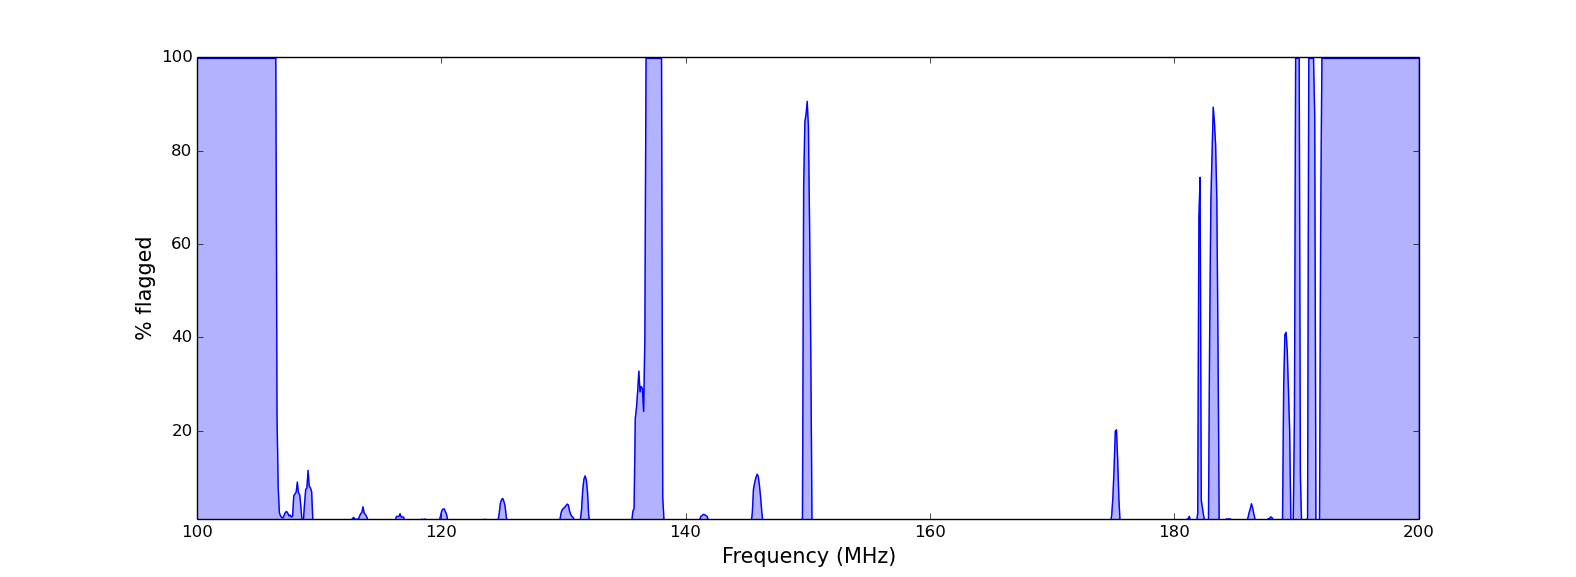
\includegraphics[width=\textwidth]{chapters/data_processing/figures/RFI_149days_freq.png}
\caption{The percentage of time that each frequency was flagged over the season.}
\label{fig:rfi_psa128_freqflags}
\end{figure}

\subsubsection*{FM Radio}

SATFA lists the frequency band 87.5--108\,MHz as available for FM radio broadcasts, leading me to postulate that the low-level RFI we observed in the 107.25	$\pm$	0.25 and 107.55	$\pm$	0.05\,MHz bands had FM radio as the leading cause. The 108.1	$\pm$	0.4 and 109	$\pm$	0.4\,MHz bands were outside of the official range, and exhibit odd temporal properties for human activity -- two peaks at midnight and 4am -- with a increasing number of flags throughout the average night (see Figure~\ref{fig:rfi_psa128_FMradio}). \\

\begin{figure}[h!]
\centering
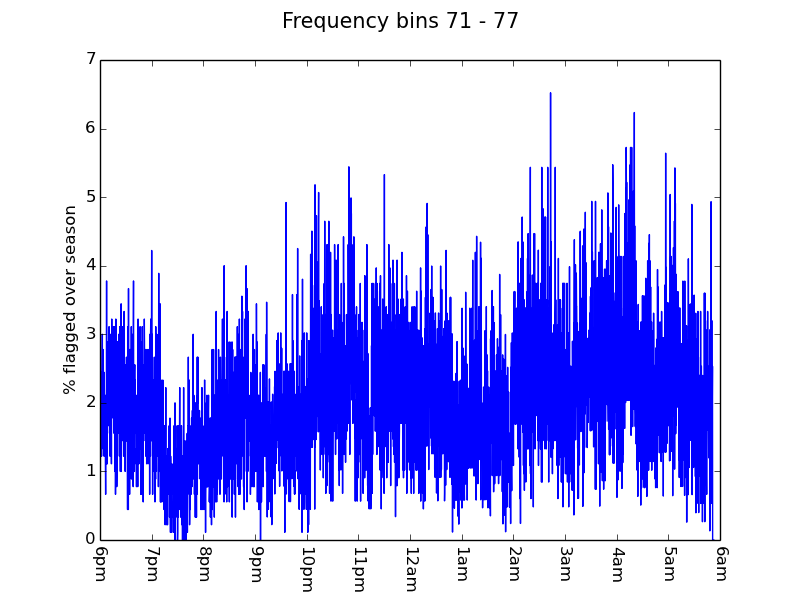
\includegraphics[width=0.4\textwidth]{chapters/data_processing/figures/FB_71_77.png}
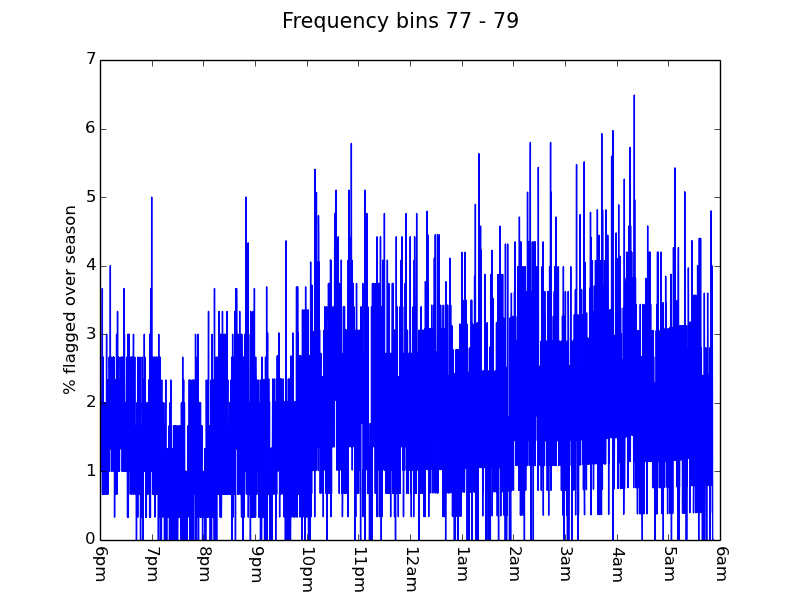
\includegraphics[width=0.4\textwidth]{chapters/data_processing/figures/FB_77_79.png}
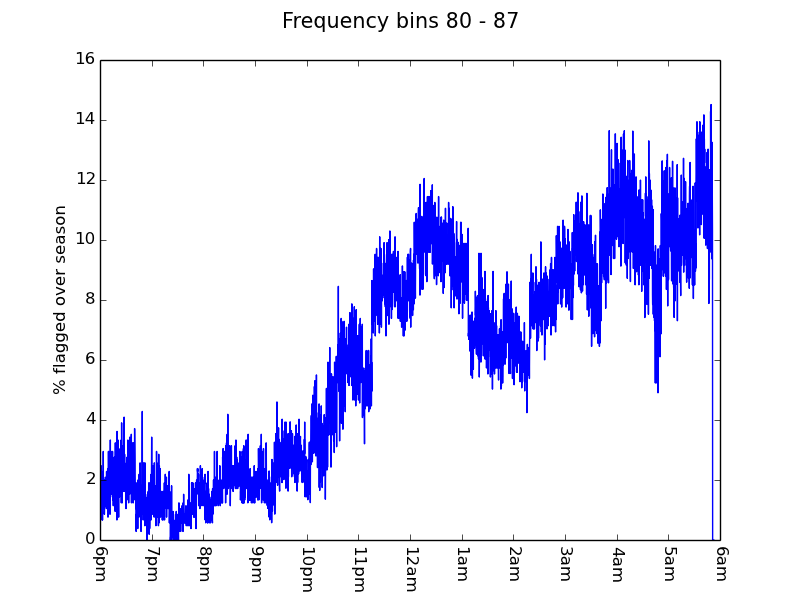
\includegraphics[width=0.4\textwidth]{chapters/data_processing/figures/FB_80_87.png}
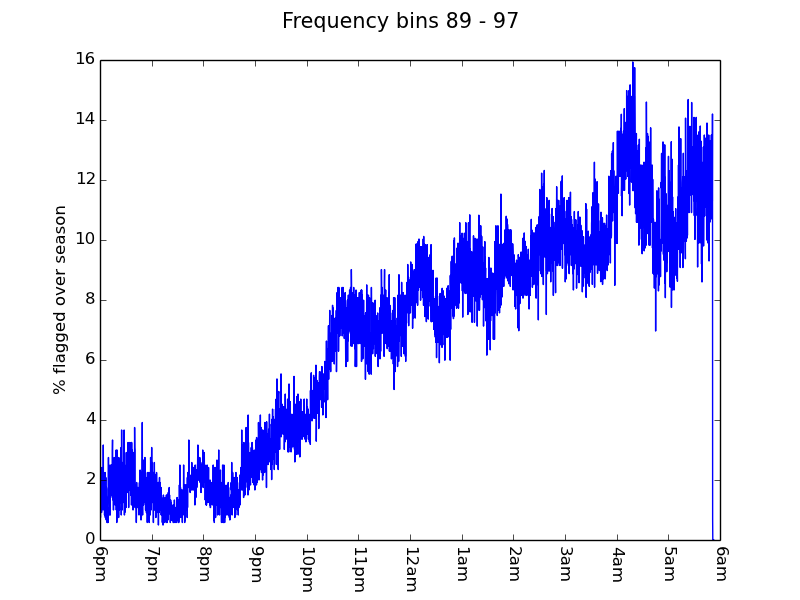
\includegraphics[width=0.4\textwidth]{chapters/data_processing/figures/FB_89_97.png}
\caption[Possible FM radio contamination.]{Possible FM radio contamination in the \textit{Top, left to right}: 107.25$\pm$0.25 and 107.55$\pm$0.05\,MHz bands, and \textit{Bottom, left to right}: 108.1$\pm$0.4 and 109$\pm$0.4\,MHz bands.}
\label{fig:rfi_psa128_FMradio}
\end{figure}

\subsubsection*{Aircraft communications}
It was difficult to argue that the 112.1$\pm$0.1\,MHz signal is caused by aircraft communications since it maintained a constant background level. However, SATFA listed this frequency as reserved for aircraft communications and it has been used in the past as a calibration frequency for aircraft instruments \cite{AircraftCalibrationFreqs}.\\

The other aircraft frequencies were obvious, because they closely traced the 2-hour flight from Cape Town to Johannesburg\footnote{Credit to Danny Jacobs for first spotting this and noting it in an internal PAPER circular in December 2009.}. 
An example (120.15$\pm$0.35\,MHz) is shown in Figure~\ref{fig:rfi_psa128_aircraft}. SATFA reserved frequencies 108--117.975\,MHz for aeronautical radionavigation and 117.975--137\,MHz for aeronautical mobile. In Table~\ref{tab:rfi_psa128} I listed 131.75$\pm$0.35\,MHz as caused by aircraft since it falls in the aeronautical mobile band, but it does not follow the flight patterns as closely as the other bands.\\

\begin{figure}[h!]
\centering
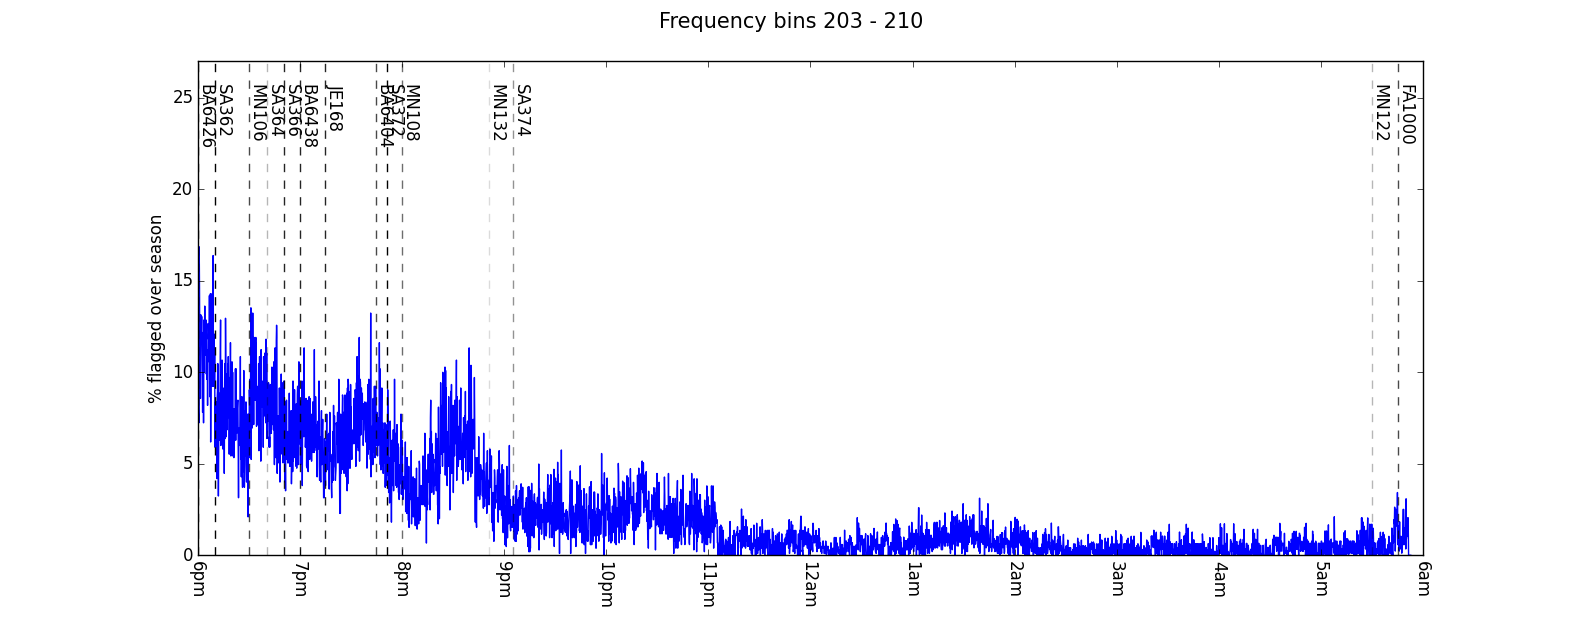
\includegraphics[width=\textwidth]{/Users/saulkohn/Documents/thesis/chapters/data_processing/figures/airlines.png}
\caption[Flights from Cape Town to Johannesburg correspond to RFI.]{
Flights from Cape Town to Johannesburg correspond to RFI in the 120.15$\pm$0.35\,MHz channels. Vertical dashed lines indicate a flight leaving Cape Town (flights from Johannesburg are roughly concurrent) and the flight code is listed. The transparency of a line is inversely proportional to how many days a week that flight is scheduled for. The flight is 2 to 2.5 hours long -- and about 2 hours after the last flight of the day, the flags fall to background level (but notably, not always to zero).}
\label{fig:rfi_psa128_aircraft}
\end{figure} 

\subsubsection*{Orbital communications}
ORBCOMM Inc.'s constellation of 29 LEO communication satellites is a well-known contaminant of the low-frequency sky, dominating over any astronomical signal at 137--138\,MHz (although each satellite emits within a 20\,kHz band). For this reason there was built-in flagging at 137.35$\pm$0.85\,MHz within the compression pipeline.

The largest contaminant without built-in flags in the pipeline were communications from the ISS. The 149.75$\pm$0.55\,MHz transmissions were semi-regular in time; they `beep'. 

Onboard the ISS are HAM radio devices. Some countries have also launched satellites with these onboard, one of the purposes of which is to provide HAM radio operators something in space to communicate with. These devices are licensed to operate at 145.2 and 145.8\,MHz, and SATFA listed the 144-146\,MHz band as reserved for `Amateur--Satellite' communications. We detected RFI at 145.85$\pm$0.45\,MHz, although strong signal across $\sim$10\% of the season that occurs 9pm-1am argues against human operation.

\subsubsection*{Mobile phones and VHF TV}
A weak RFI signal at 141.45$\pm$0.35\,MHz was within the `mobile 1 BTX'  and aeronautical mobile band in SATFA, but other than this single listing I did not build a strong case for the signal's cause.

VHF TV is broadcast over specifically-spaced video and audio frequencies. The strong signals at 183.2$\pm$0.5\,MHz and 189.15$\pm$0.35\,MHz had almost identical gradients for the percentage of flagging as a function of time of night. These frequencies corresponded exactly to Channel 5 of South African System I 625-line VHF TV signals for video and audio transmission, respectively. Similarly, the weaker signals at 175.15$\pm$0.35	 and 181.15$\pm$0.15\,MHz corresponded to Channel 4's video and audio transmission, respectively, but they did not share the same temporal properties.

\subsubsection*{Unidentified sources}

There were 5 RFI frequencies in the averaged data that I could not identify the sources of:  weak emissions (flagged $<5\%$ of the season) at 114.05$\pm$0.85, 116.55$\pm$0.35, 130.25$\pm$0.55 and 186.25$\pm$0.35\,MHz, and one strong emission at 182.15$\pm$0.35\,MHz. The variation of each source with time is shown in Figure~\ref{fig:rfi_psa128_unidentified}. The 186.25$\pm$0.35\,MHz had a sharp turn-off around 9:45pm each night, suggesting that it originated from some kind of automated device.\\

\begin{figure}[h!]
\centering
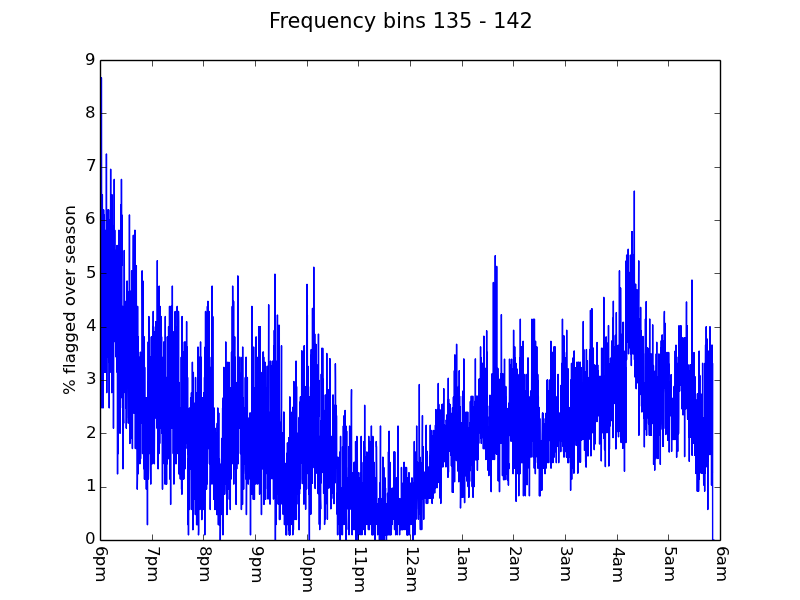
\includegraphics[width=0.4\textwidth]{chapters/data_processing/figures/FB_135_142.png}
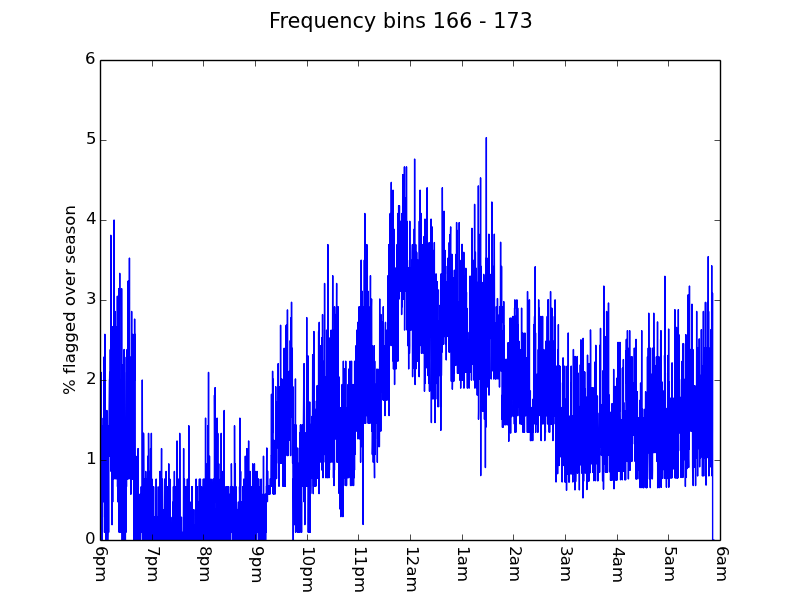
\includegraphics[width=0.4\textwidth]{chapters/data_processing/figures/FB_166_173.png}
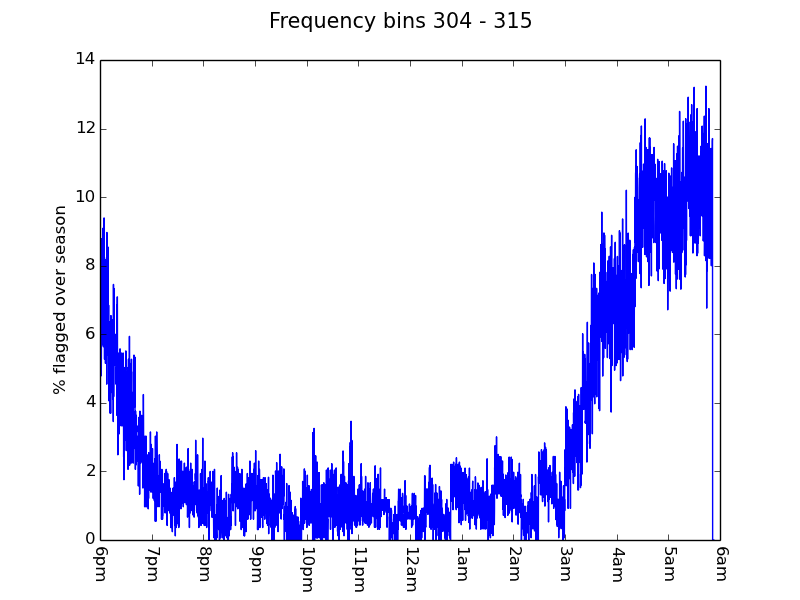
\includegraphics[width=0.4\textwidth]{chapters/data_processing/figures/FB_304_315.png}
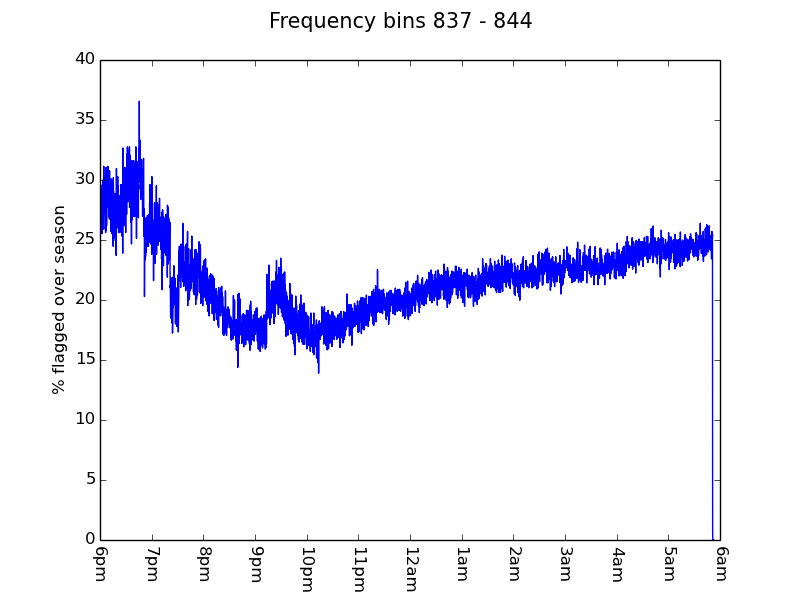
\includegraphics[width=0.4\textwidth]{chapters/data_processing/figures/FB_837_844.png}
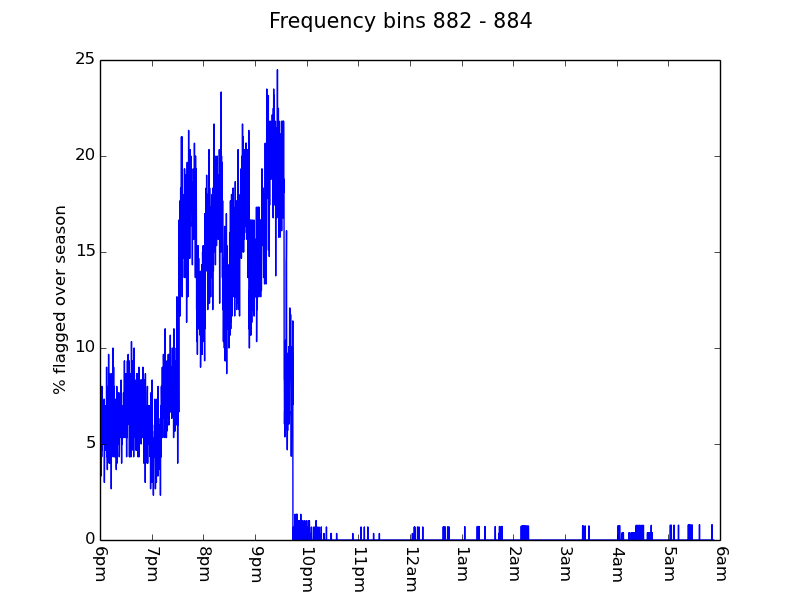
\includegraphics[width=0.4\textwidth]{chapters/data_processing/figures/FB_882_884.png}
\caption[The temporal profile of the 5 RFI frequencies with unidentified causes.]{The temporal profile of the 5 RFI frequencies with unidentified causes. \textit{Top, left to right:} 114.05$\pm$0.85 and 116.55$\pm$0.35\,MHz. \textit{Middle, left to right:} 130.25$\pm$0.55 and 182.15$\pm$0.35\,MHz. \textit{Bottom:} 186.25$\pm$0.35\,MHz. The 182.15$\pm$0.35\,MHz frequency is flagged a large amount of the time, making it our most-offending unidentified source.}
\label{fig:rfi_psa128_unidentified}
\end{figure}

\subsubsection{Individual Properties}
\label{subsubsec:indivprops}

Using the flags per night, I was able to assess the total number of flags as a percentage of the waterfall (i.e. $N_{\rm flags}/(3920\times1024)$). The average flagging per night was 19.2$\pm$0.5\%, which was dominated by the permanent flagging of ORBCOMM and band edges. Four nights deviated from the average by a $\geq 2\sigma$ excess: JDs 2456965, 2456732, 2456958 and 2457038. Their flag waterfalls are shown in Figure~\ref{fig:rfi_psa128_worst} (2456732, 2456958 and 2457038) and Figure~\ref{fig:rfi_psa128_wandering} (2456965). While the strange nature of night 2456965 is discussed below, the three others followed the pattern of having strong contamination from FM and aircraft communication bands, but also had broadband `pulses' up to about 20 minutes in length. The source of these broadband pulses is not well understood, although it was clear that ORBCOMM tends to spill outside of its allocated band on occasion.

\begin{figure}[h!]
\centering
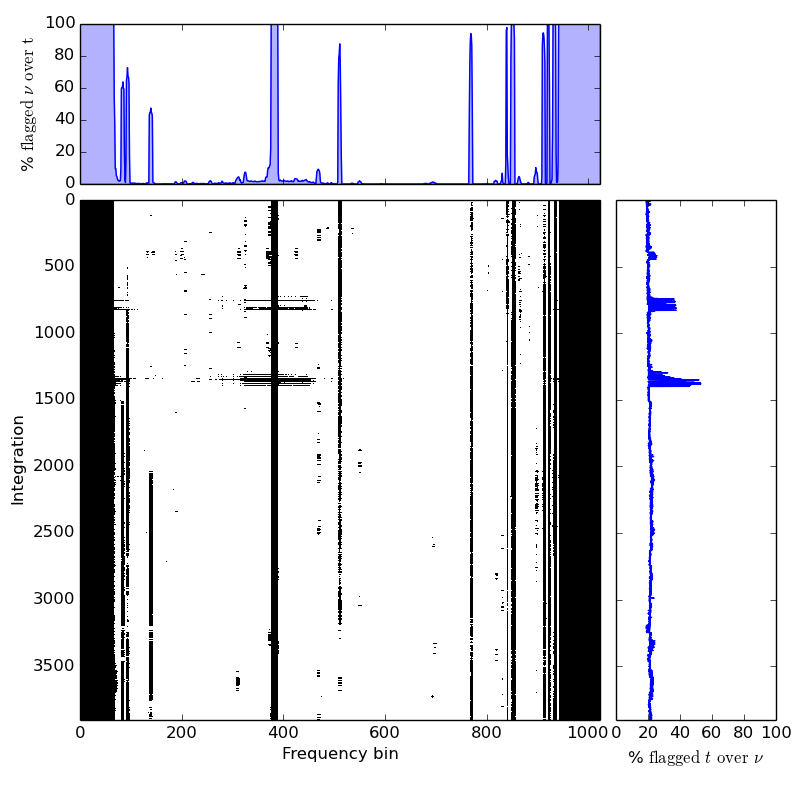
\includegraphics[width=0.3\textwidth]{chapters/data_processing/figures/2456732RFI.png}
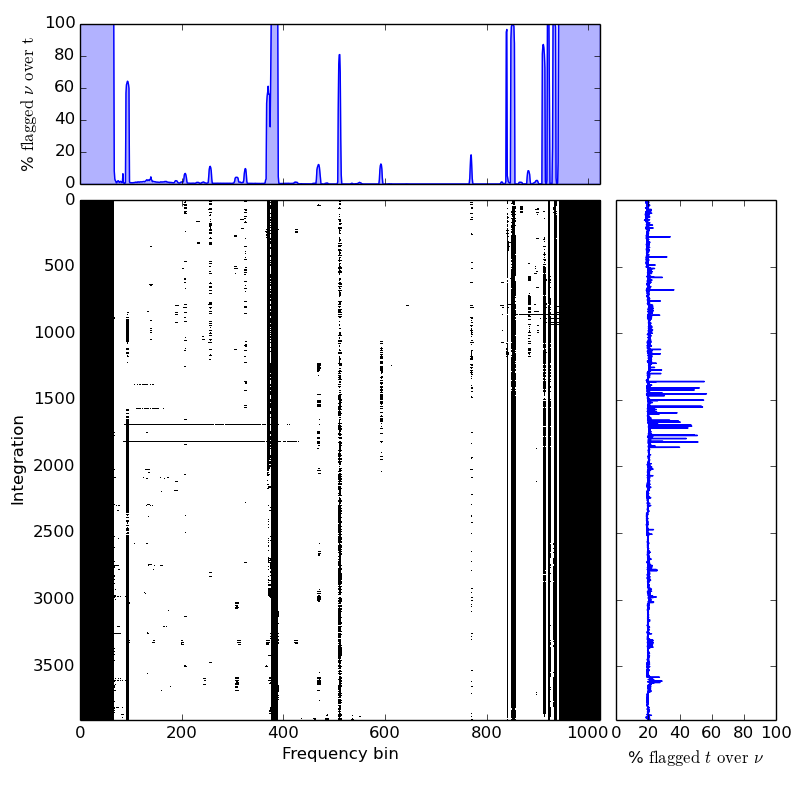
\includegraphics[width=0.3\textwidth]{chapters/data_processing/figures/2456958RFI.png}
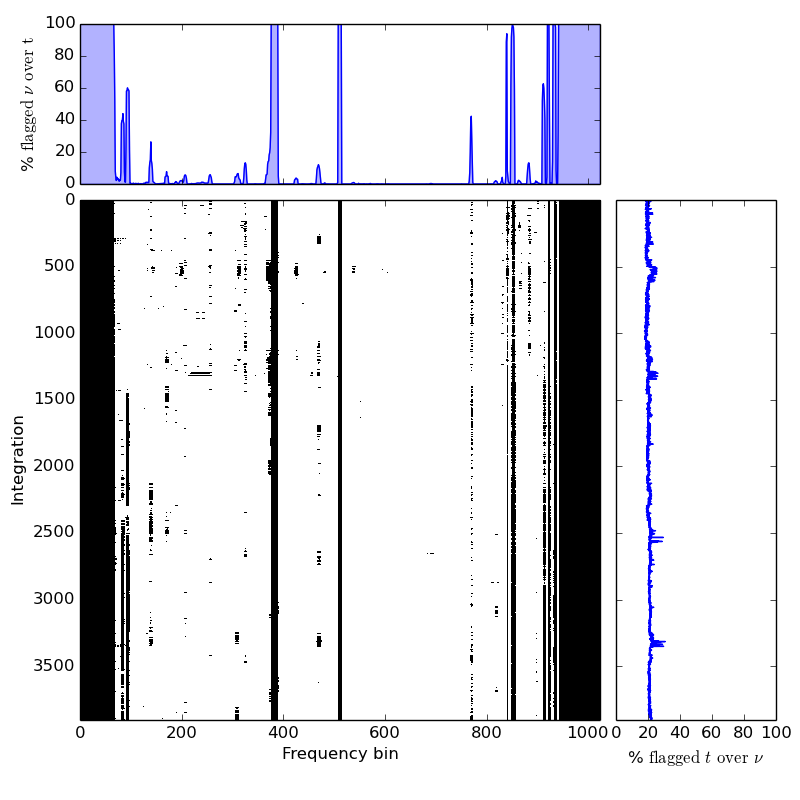
\includegraphics[width=0.3\textwidth]{chapters/data_processing/figures/2457038RFI.png}
\caption[Waterfalls of RFI flags for nights 2456732, 2456958 and 2457038.]{\textit{Left to right:} waterfalls of flags for nights 2456732, 2456958 and 2457038. These three nights, along with 2456965, are $>$20.2\% flagged; $>2\sigma$ above the average flagging amount per night.}
\label{fig:rfi_psa128_worst}
\end{figure}


JD 2456965 was easily the worst offender, and it exhibited a strange signal that wanders in frequency and time close to the ISS band. An event of note on this date (23rd November 2014) was a Soyuz FG launch that docked with the ISS -- this may have been a signature of their transmissions\footnote{The internet also suggests... less plausible explanations: \url{https://www.youtube.com/watch?t=11&v=VtZx8iPO4zs}. }.
Similar signals were seen on 2456898 (28th August 2014; although only at the beginning of the night) and 2456924 (23rd September 2014). There was no listed orbital or suborbital activity for 2456898. There was an US ICBM test off of the coast of Virginia on 2456924, but this was probably not the cause of the RFI. The flag waterfalls for these nights are shown in Figure~\ref{fig:rfi_psa128_wandering}.\\

\begin{figure}[h!]
\centering
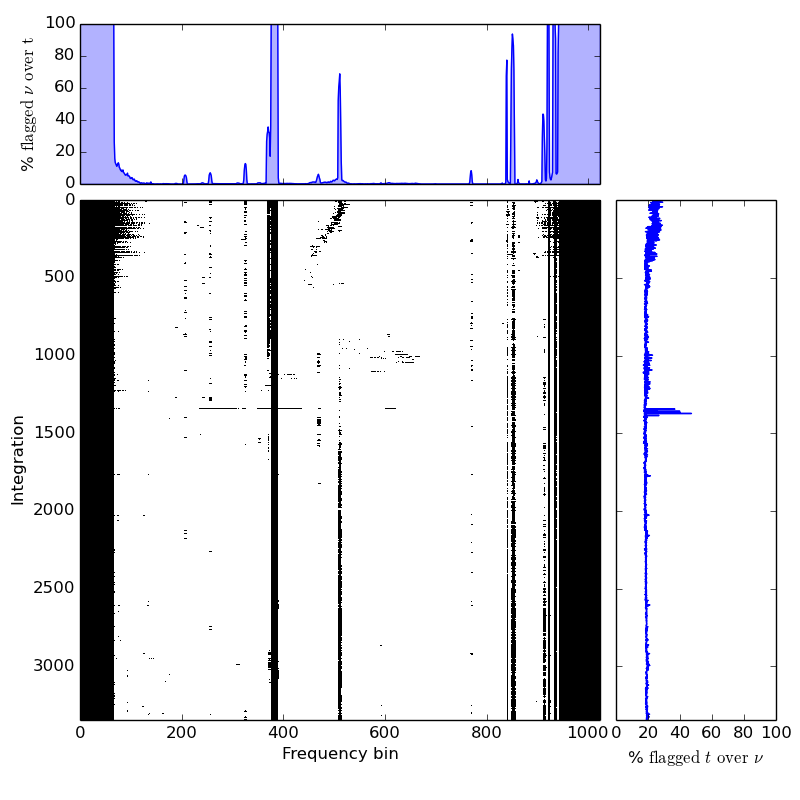
\includegraphics[width=0.3\textwidth]{chapters/data_processing/figures/2456898RFI.png}
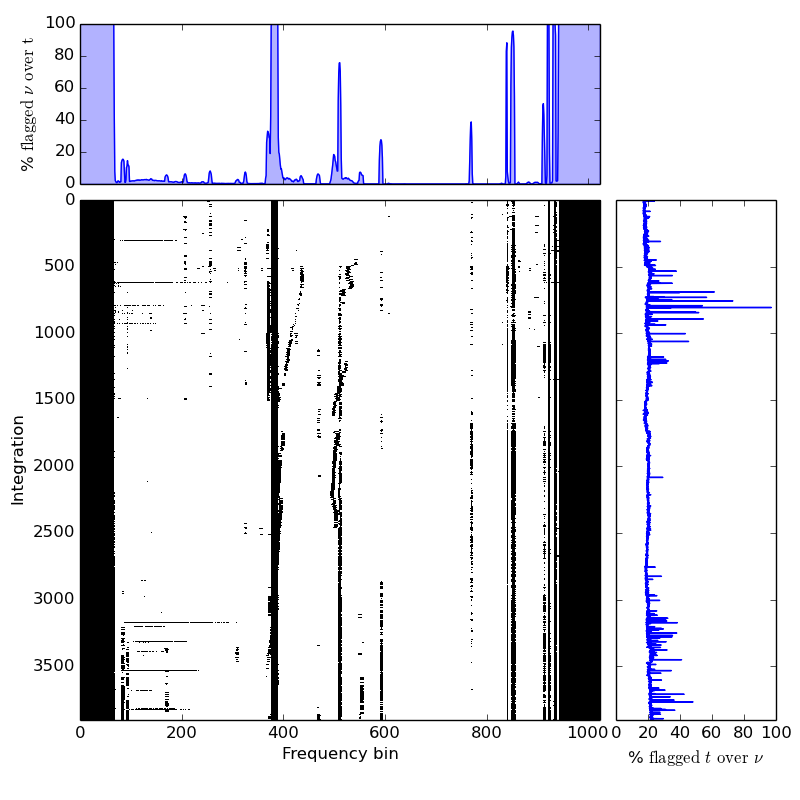
\includegraphics[width=0.3\textwidth]{chapters/data_processing/figures/2456924RFI.png}
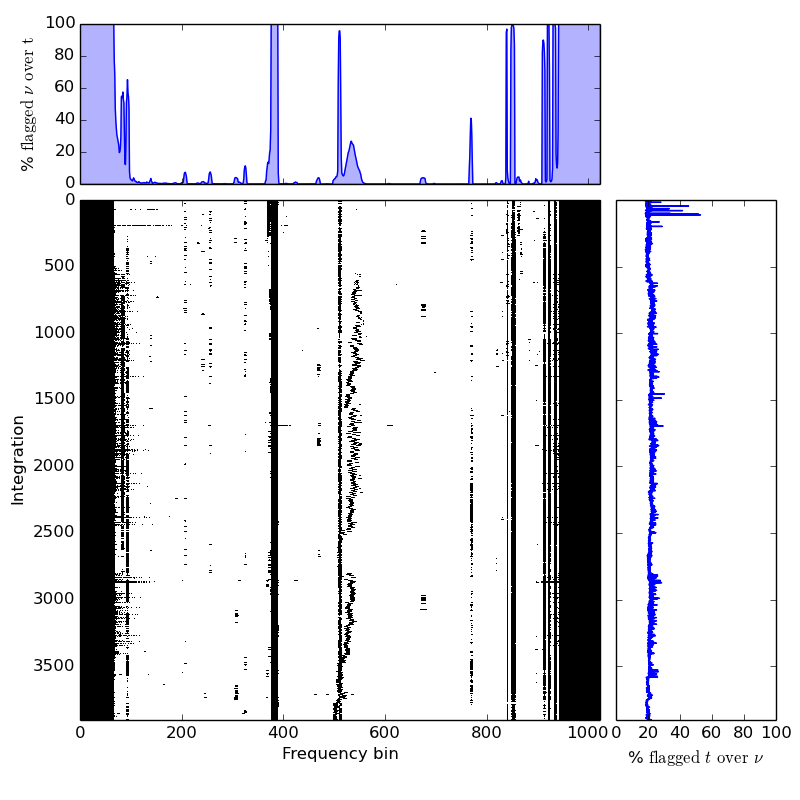
\includegraphics[width=0.3\textwidth]{chapters/data_processing/figures/2456965RFI.png}
\caption[Waterfalls of RFI flags for nights 2456898, 2456924 and 2456965]{\textit{Left to right:} waterfalls of flags for nights 2456898, 2456924 and 2456965. These three nights exhibit a strange behaviour of RFI that changes in frequency and time. JD 2456965 is by far the worst, and during this night as well as 2456898, we see a broadband `comb' of flagged frequencies near the band edges}
\label{fig:rfi_psa128_wandering}
\end{figure}

Another property that the flag waterfalls in Figures~\ref{fig:rfi_psa128_worst} and \ref{fig:rfi_psa128_wandering} highlight is the presence of broadband RFI signals, typically present at frequencies lower than the ORBCOMM band. However, while we flagged at the low-end of the band (which had higher noise levels to begin with), it is likely that such broadband pulses dominated the band at those times, and that we failed to flag all of the integrations. Our flagging routine \textit{xrfi\_simple.py} does contain a thresholding option for flagging the entire integration given some arbitrary number of frequencies flagged during that integration: some experimentation will be required to decide if that threshold should change.

\subsubsection{Discussion}
\label{subsubsec:rfi_paper128_conc}

Based on my findings, I was able to recommend some actions that could be taken in the KRQZ to enable better measurements:
\begin{itemize}
\item  Steps to reduce and ideally eliminate the VHF TV transmissions in the area would be very helpful, since these were clearly interfering with our measurements in the high-end of the band.
\item The ISS 149.75$\pm$0.55\,MHz band should be permanently flagged within the compression pipeline.
\item Pursuing re-routing of flight paths will not do much to help: we see aircraft signals for the duration of their flight, not just when they're over the Karoo.
\item A lower threshold for identifying broadband RFI should be investigated.
\end{itemize}

A new, lower-frequency feed is currently under development by the HERA analog group. This would nominally allow measurements to be taken in the range 50--250\,MHz, allowing science observations of the Dark Ages and the post-reionization Universe. It should be noted that at the lowest frequencies FM radio will be a constant harassment to these measurements. At the higher frequencies, VHF TV will be the primary contaminant, but should be much easier to remove as it is both narrow-band and within the KRQZ's power to shut off.

\subsection{HERA-19 and PAPER-19}
\label{subsec:rfi_hera19paper19}

The HERA-19 IDR1 consisted of four subarrays: the HERA-19 hexagon of dishes (the `HERA Hex'), a hexagon of 19 PAPER dipoles in the exact positions of not-yet-constructed HERA dishes (the `PAPER Hex'), an imaging array and an experimental array for polarization measurements. I will concentrate on the two Hexes in this Section. I analyzed RFI as flagged in the linear \textit{xx}-polarization only. Asymmetric beams can in principle receive different RFI events for different linear polarizations, but analysis of that was outside the scope of this diagnostic study.

IDR1 consisted of one `golden day', JD 2457458. This ran from 6pm on March 10th 2016 to 6am the following day. This gave, per baseline, roughly 4000 integrations of 10 seconds each over 1024, 100~kHz frequency channels from 100 to 200~MHz.

In order to flag RFI I used the {\tt aipy} script \textit{xrfi\_simple.py}. I took the union of all baseline flags as data to analyze. Unlike in Section~\ref{subsec:rfi_paper128}, these data did not have a-priori flagging of band edges, which allowed me to make a more complete study of RFI in the HERA band. I did have to implement custom flags in order to get more than a zeroth-order view of the RFI (since these would dominate the flagging routine unless they are flagged already), but my results from Section~\ref{subsec:rfi_paper128}  gave a better idea of what was flagged to get there. 

Below I present measurements of high-power, mostly narrow-band RFI channels as flagged in HERA Hex data and PAPER Hex data separately. In both cases, I was able to list any channels that are flagged for $\geqslant 1\%$ of the night. I could then compare the flagging Hex-to-Hex, and to PAPER-128.

\subsubsection{HERA Hex RFI}
\label{subsubsec:rfi_herahex}

Table~\ref{tab:rfi_herahex} shows all narrowband frequency ranges flagged in HERA-19 visibilities, with columns of the frequency range in MHz, \% flagging over time, plausible identification, whether or not it was identified in PAPER-128 data, and other notes (often details of the possible identification). Frequencies with 100\% flagging indicate manual flags required for {\tt xrfi\_simple} to work on the rest of the channels. 

Clearly, the low-end of the band was swamped by FM radio broadcasts. One notable frequency was the 109.2$\pm$0.3~MHz band, which was heavily flagged in HERA visibilities, but was only flagged a few percent in PAPER-128 data.

As seen before, ORBCOMM satellite emissions spilled out of their allocated 137-138~MHz band down to 136.3~MHz.

There were many narrowband RFI channels, across the band, that PAPER-128 did not pick-up. Most of these were flagged only at low levels, with two exceptions: 111.3$\pm$0.2~MHz and 113.5$\pm$0.1~MHz. Both of these were in the aircraft navigation band. There is some evidence \citep{airforce} that 111.3~MHz band is fir air force communications. The 113.5~MHz band is a known band for radionavigation beacons \citep[`VOR navaids'][]{navaid}.

A particularly annoying `new' emitter was in the 153.8$\pm$0.2~MHz region, which is close to the center of our nominal EoR band. It could correspond to mobile phones being used close to site.

\begin{deluxetable}{lllll}				
\centering														
\label{tab:rfi_herahex}
\tablewidth{0pt}
\tablecaption{RFI as flagged by HERA}
\tabletypesize{\footnotesize}
\tablehead{
\colhead{$\nu$} & \colhead{Flagged} & \colhead{Cause} & \colhead{Seen by} & \colhead{Notes} \\
\colhead{MHz} & \colhead{\%} & \colhead{(Possible)} & \colhead{PAPER-128} &\colhead{} \\
}
\startdata													
100.7	$\pm$	0.2	&	50	&	FM Radio	&	n/a	&	RSG ``Dis Die Een'' Prieska		\\
101.5	$\pm$	0.3	&	36	&	FM Radio	&	n/a	&	RSG ``Dis Die Een'' Calvinia	\\
102.4	$\pm$	0.1	&	100	&	FM Radio	&	n/a	&	RSG ``Dis Die Een'' Carnarvon	\\
102.8	$\pm$	0.3	&	57	&	FM Radio	&	n/a	&	RSG ``Dis Die Een'' Pofadder	\\
104.2	$\pm$	0.1	&	100	&	FM Radio	&	n/a	&	SAfm Prieska	\\
105.1	$\pm$	0.2	&	100	&	FM Radio	&	n/a	&	SAfm Calvinia	\\
106.2	$\pm$	0.3	&	100	&	FM Radio	&	n/a	&	SAfm Carnarvon	\\
106.9	$\pm$	0.1	&	15	&	FM Radio	&	n/a	&	Sentech	\\
107.2	$\pm$	0.1	&	18	&	FM Radio	&	Yes	&		\\
107.8	$\pm$	0.2	&	15	&	FM Radio	&	Yes	&		\\													
108.3	$\pm$	0.1	&	31	&	FM Radio?	&	Yes	&			\\
109.2	$\pm$	0.3	&	93	&	FM Radio?	&	Yes...&	...but not to this degree	\\
111.3	$\pm$	0.2	&	25	&	Air force?	&	No	&		\\
112.5	$\pm$	0.1	&	5	    &	Aircraft?	&	No	&	\\
113.5	$\pm$	0.1	&	21	&	Aircraft    &	No	&	VOR navaids		\\
115.5	$\pm$	0.1	&	3	    &	Navaids?	    &	No	&	\\
115.9	$\pm$	0.1	&	3	    &	Navaids?	    &	No	&	\\
116.6	$\pm$	0.2	&	9	   &	Aircraft?	    &	Yes	&	VOR-DME navaids		\\
120.1	$\pm$	0.2	&	5	&	Aircraft	&	Yes	&	CPT$<->$JNB		\\
125.0$\pm$	0.2	&	6	&	Aircraft	&	Yes	&	CPT$<->$JNB		\\
130.0	$\pm$	0.2	&	4	&	Aircraft	&	No	&	Communication		\\
131.6	$\pm$	0.2	&	15	&	Aircraft	&	Yes	&	KLM OPS		\\
136.4	$\pm$	0.1	&	9	&	ORBCOMM	&	Yes	&					\\
136.7	$\pm$	0.1	&	10	&	ORBCOMM	&	Yes	&					\\
137.4	$\pm$	0.4	&	100	&	ORBCOMM	&	Yes	&				\\
145.7	$\pm$	0.4	&	18	&	ISS/Amateur Radio band	&	Yes	&			\\
149.9	$\pm$	0.1	&	100	&	ISS	&	Yes	&			\\
153.8	$\pm$	0.2	&	7	&	Mobile phones?	&	No	&			\\
175.0	$\pm$	0.1	&	100	&	VHF TV	&	Yes	&	Channel 4 Video		\\
178.3	$\pm$	0.2	&	8	&	VHF TV	&	No	&	Channel 7?		\\
181.2	$\pm$	0.1	&	100	&	VHF TV	&	Yes	&	Channel 4 Audio		\\
182.2  $\pm$	0.2	&	9	&		&	Yes	&			\\
183.5	$\pm$	0.6	&	100	&	VHF TV	&	Yes	&	Channel 5 Video		\\
184.1	$\pm$	0.1	&	2	&	VHF TV?	&	Yes	&	Channel 5?	\\
184.7	$\pm$	0.1	&	6	&	Broadcasting	&	No	&		\\
187.8	$\pm$	0.1	&	4	&		&	No	&		\\
189.1	$\pm$	0.1	&	52	&	VHF TV	&	Yes	&	Channel 5 Audio	\\
190.1	$\pm$	0.3	&	13	&		&	n/a	&		\\
191.1	$\pm$	0.1	&	100	&	VHF TV	&	n/a	&	Channel 7		\\
197.2	$\pm$	0.2	&	18	&		&	n/a	&		\\
199.4	$\pm$	0.5	&	100	&	BAND EDGE	&	n/a	&		\\
\enddata
\end{deluxetable}

\subsubsection{PAPER Hex RFI}
\label{subsubsec:rfi_paperhex}

Table~\ref{tab:rfi_paperhex} has the same description as Table~\ref{tab:rfi_herahex}, but for the PAPER Hex. There were far fewer RFI frequencies flagged in PAPER visibilities, almost all of which were seen by HERA. The only RFI seen by the PAPER Hex and not the HERA Hex was the 123.5$\pm$0.1~MHz emission, which I could find a plausible identification for.

\begin{deluxetable}{lllll}													
\centering														
\label{tab:rfi_paperhex}
\tablewidth{0pt}
\tablecaption{RFI as flagged by the PAPER Hex}	
\tabletypesize{\footnotesize}
\tablehead{
\colhead{$\nu$} & \colhead{Flagged} & \colhead{Cause} & \colhead{Seen by} & \colhead{Notes} \\
\colhead{MHz} & \colhead{\%} & \colhead{(Possible)} & \colhead{PAPER-128} &\colhead{} \\
}
\startdata	
100.0	$\pm$	0.1	&	100	&	BAND EDGE	&	n/a	&		\\		
100.7	$\pm$	0.1	&	11	&	FM Radio	&	n/a	&	RSG ``Dis Die Een'' Calvinia			\\		
101.6	$\pm$	0.2	&	6	&	FM Radio	&	n/a	&	RSG ``Dis Die Een'' Calvinia			\\		
102.4	$\pm$	0.1	&	100	&	FM Radio	&	n/a	&	RSG ``Dis Die Een'' Carnarvon		\\		
102.7	$\pm$	0.1&	100	&	FM Radio	&	n/a	&	RSG ``Dis Die Een'' Pofadder		\\		
104.2	$\pm$	0.2	&	100	&	FM Radio	&	n/a	&	SAfm Prieska		\\		
105.1	$\pm$	0.2	&	100	&	FM Radio	&	n/a	&	SAfm Calvinia	\\		
106.2	$\pm$	0.3	&	100	&	FM Radio	&	n/a	&	SAfm Carnarvon	\\		
																
108.2	$\pm$	0.1	&	3	&	FM Radio?	&	Yes	&		\\		
109.1	$\pm$	0.1  &	26	&	FM Radio?	&	Yes	&		\\		
113.6	$\pm$	0.1	&	2	&	Airplane Communications	&	No	&	VOR navaid			\\		
																
120.2	$\pm$	0.3	&	3	&	Aircraft	&	Yes	&	CPT$<->$JNB		\\		
123.5	$\pm$	0.1	&	1	&		&	No	&	Not seen by HERA			\\		
125.0	$\pm$	0.2	&	6	&	Aircraft	&	Yes	&	CPT$<->$JNB		\\		
130.0	$\pm$	0.3	&	3	&		&	No	&			\\		
131.7	$\pm$	0.2	&	14	&	Aircraft	&	Yes	&				\\		
136.4	$\pm$	0.2	&	6	&	ORBCOMM	&	Yes	&					\\		
136.7	$\pm$	0.2	&	6	&	ORBCOMM	&	Yes	&				\\		
															
137.4	$\pm$	0.4	&	100	&	ORBCOMM	&	Yes	&				\\		
145.8	$\pm$	0.3	&	14	&	ISS/Amateur Radio band	&	Yes	&			\\		
149.9	$\pm$	0.1	&	100	&	ISS	&	Yes	&			\\		
153.8	$\pm$	0.2	&	3	&	Single frequency mobile phones?	&	No	&				\\		
																
175.1	$\pm$	0.2	&	100	&	VHF TV	&	Yes	&	Channel 4 Video				\\		
178.3	$\pm$	0.2	&	100	&	VHF TV	&	No	&	Channel 7?		\\		
181.2	$\pm$	0.1	&	100	&	VHF TV	&	Yes	&	Channel 4 Audio	\\		
183.2	$\pm$	0.2	&	100	&	VHF TV	&	Yes	&	Channel 5 Video			\\		
189.2	$\pm$	0.1	&	100	&	VHF TV	&	Yes	&	Channel 5 Audio			\\		
191.2	$\pm$	0.1	&	100	&	VHF TV	&	n/a	&	Channel 7			\\		
199.8	$\pm$	0.2	&	100	&	BAND EDGE	&	n/a	&			\\
\enddata
\end{deluxetable}

\subsubsection{Hex-to-Hex Comparisons}
\label{subsubsec:hex2hex_comparison}

As mentioned above, the PAPER Hex saw far fewer narrowband RFI channels than HERA does. This highlighted an interesting trade-off between dipoles and dishes: at first glance, one might have expected PAPER dipoles to be more susceptible to RFI given their broader effective beams. However, HERA dipoles are lifted several meters above the ground, and this change in height may have been the source of the greater susceptibility to RFI. RFI comes from the horizon, which would be more easily received in the far sidelobes of the beam.

\begin{figure}[h!]
\centering
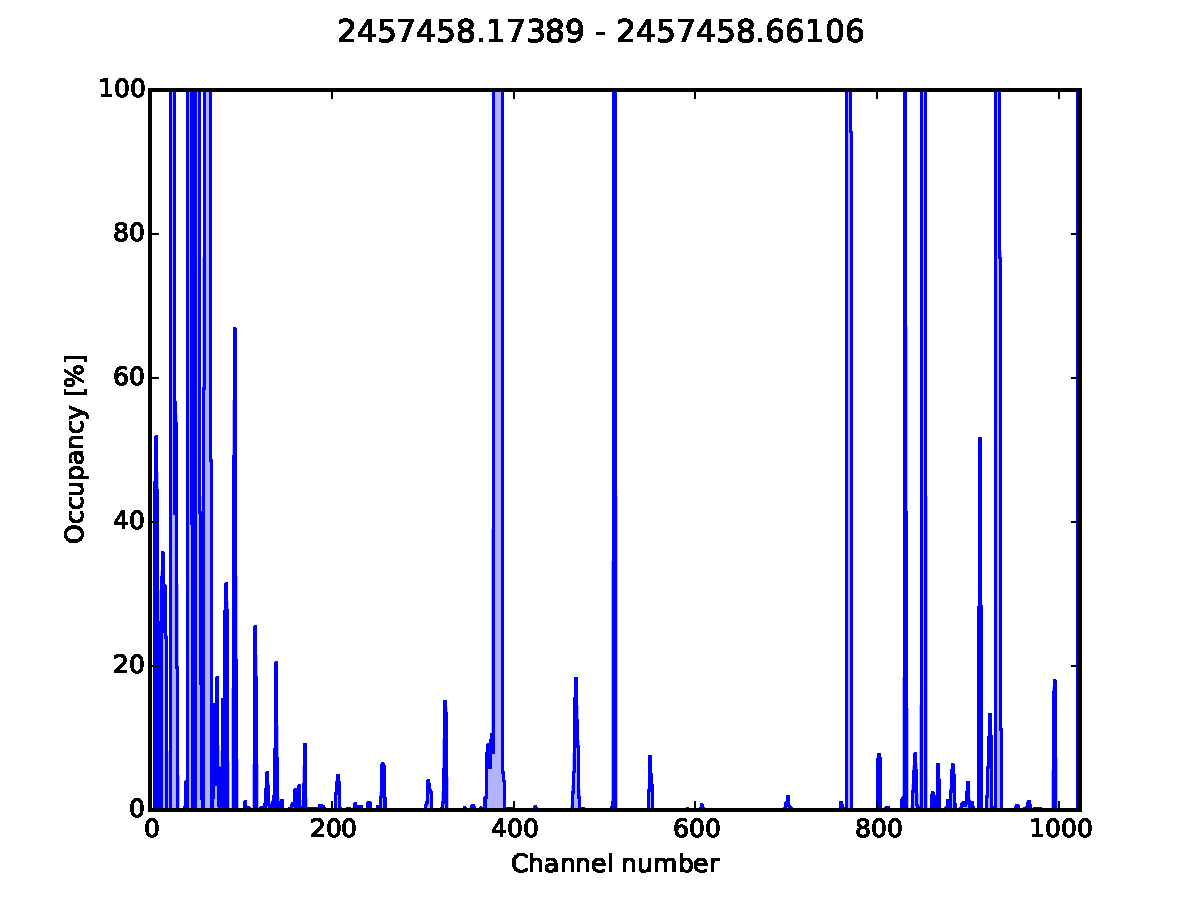
\includegraphics[width=0.45\textwidth]{chapters/data_processing/figures/RFI_HH_spec.pdf}
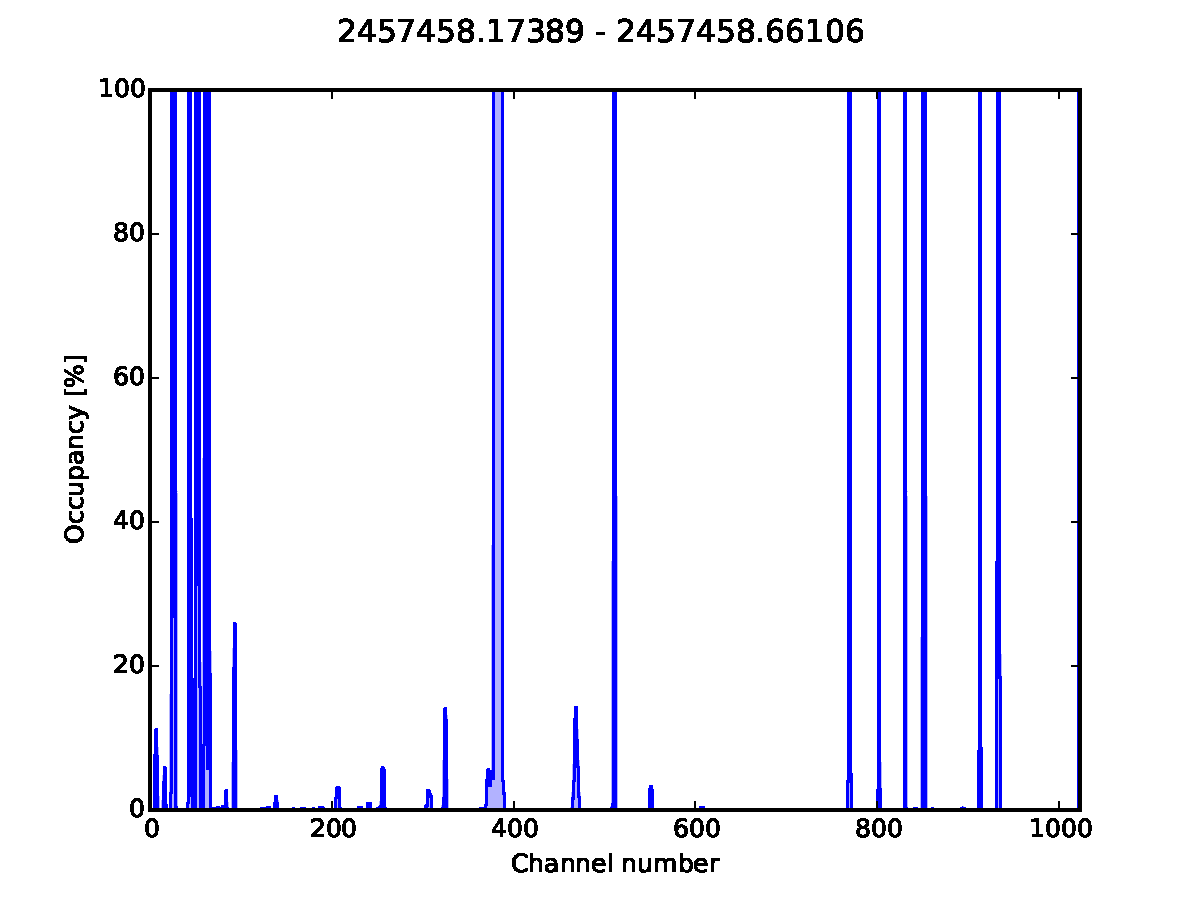
\includegraphics[width=0.45\textwidth]{chapters/data_processing/figures/RFI_PH_spec.pdf}
\caption[Frequency vs. percentage flagging for the HERA Hex and PAPER Hex.]{Frequency vs. percentage flagging for the HERA Hex (\textit{left}) and PAPER Hex (\textit{right}). Any band with greater than 1\% flagging is reported in Tables~\ref{tab:rfi_herahex} and \ref{tab:rfi_paperhex}.}
\label{fig:rfi_spec_hex_comparison}
\end{figure}

Even for the RFI channels they did share, HERA flagged them more often. Taking the difference in percentage-flagging for the common RFI channels (think of the left panel subtracted from the right panel for common channels in Figure~\ref{fig:rfi_spec_hex_comparison}), those channels had an average of 8\% more flagging in HERA visibilities. The difference was particularly high in the aeronautical radionavigation bands, where HERA had on average 38\% more flagging than the PAPER Hex.

Figure~\ref{fig:rfi_hex_waterfalls} shows the flags on a per-sample basis (these were averaged over time to create Figure~\ref{fig:rfi_spec_hex_comparison}). Most apparent was the occupancy of the HERA plot compared to the PAPER Hex one. An important component of this plot is the averages over frequency in the right-hand panels. We saw that the average flagging for a given time sample was about 5\% higher for HERA than for the PAPER Hex, mostly due to the higher occupancy of the FM band. But we also saw something new; HERA appeared to be much more sensitive to broadband bursts of RFI. The PAPER Hex caught one of these events (around 1.30am SAST) at high significance, but most of them hardly rose above average flagging. HERA saw five to seven bursts across the night. 

\begin{figure}
\centering
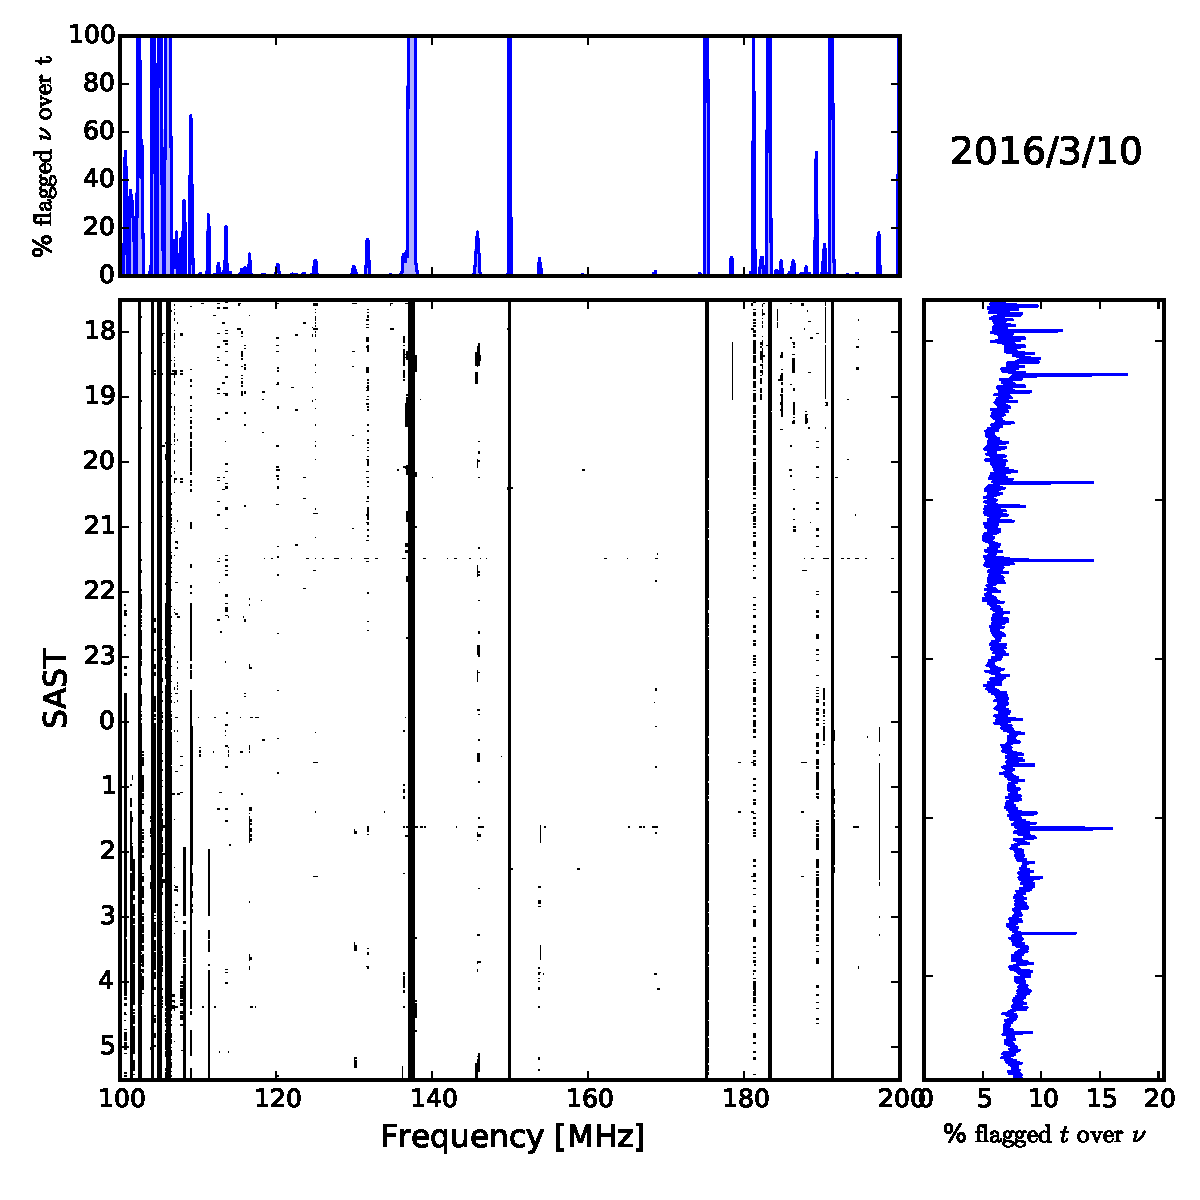
\includegraphics[width=0.45\textwidth]{chapters/data_processing/figures/RFI_HH_wf_tzoom.pdf}
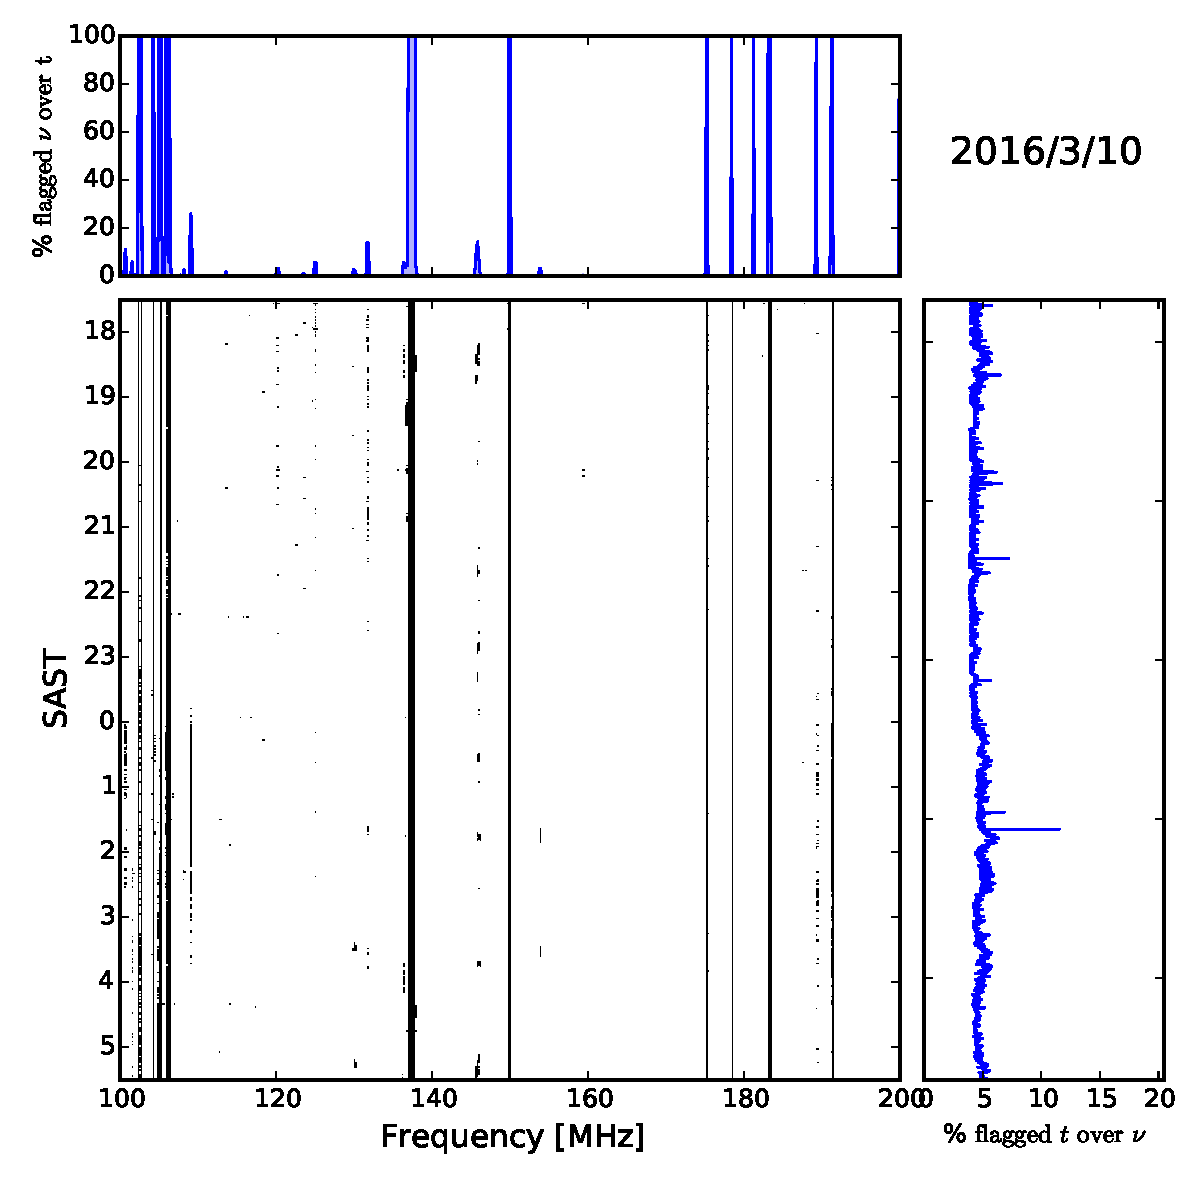
\includegraphics[width=0.45\textwidth]{chapters/data_processing/figures/RFI_PH_wf_tzoom.pdf}
\caption[RFI flag waterfalls of frequency vs. South Africa Standard Time for the HERA Hex and PAPER Hex.]{RFI flag waterfalls of frequency vs. South Africa Standard Time for the HERA Hex (\textit{left}) and PAPER Hex (\textit{right}). The top panels show the average over time (identical to Figure~\ref{fig:rfi_spec_hex_comparison}), while the right panels show the average over frequency.}
\label{fig:rfi_hex_waterfalls}
\end{figure}

\subsubsection{Comparison PAPER-128 stacked flags}
Section~\ref{subsec:rfi_paper128} presented RFI flags stacked over 150 days of observations. This method washed-out single events that effect analysis on a single-night basis, but was sensitive to repeatedly offending frequencies. Due to the PAPER-128 analysis pipeline, many channels were automatically flagged (particularly large portions of the band edges), which artificially boosted the average flagging per time and did not allow for closer inspection of the ends of the band. There was some evidence of broadband emission (see Figure~\ref{fig:rfi_psa128_waterfall}) but the band was largely free of RFI in the middle of the night. Obviously, the data presented in this section shows a less-clean band, but it also only concentrated on a single night's data, so it may be that IDR1 was conspicuous compared to an `average' night of observations.

Traits shared between the two analyses were:
\begin{itemize}
\item Aircraft communications disrupting data until around local midnight.
\item ORBCOMM spilling out of it's band.
\item VHF TV frequencies emitting throughout the night in the high end of the band.
\end{itemize} 

Table~\ref{tab:rfi_herahex} highlighted many frequencies seen by HERA and not by PAPER-128. Again, given the fact that flags were stacked and averaged in Section~\ref{subsec:rfi_paper128}, these may not have been `new', but they could have been. Particularly conspicuous were the emissions in the aeronautical radionavigation band.

\subsubsection{Discussion}
\label{subsubsec:rfi_herapaper_conc}

I have presented a first look at RFI in HERA-19 Commissioning data. Probably due to the height of the receiving element on HERA versus PAPER dipoles, much more RFI was apparent, especially on the low and high ends of the band. Luckily, the EoR band was largely clean of RFI, except for an emitter at about 154~MHz, which could have corresponded to single-frequency mobile phone communications. Such communications are officially banned in the SKA Radio Quiet Zone \citep{SAKRQZ}, which HERA is in the center of.

Only looking at a single night of RFI flags limited the predictive power of this study. More data will be required to establish whether or not this is level of RFI was `normal'. Broadband RFI bursts require closer investigation.

Efforts to extend the HERA band to lower and possibly higher frequencies are currently under way. The FM radio band extends to around 65~MHz, while the VHF TV band extends to around 230~MHz, so the RFI environment should be a consideration for these efforts.

Meanwhile, I note that the RFI flagging routine used here, {\tt xrfi\_simple}, is indeed `simple'. More advanced RFI flagging algorithms such as {\tt AOFlagger} \citep{AOflag} should be tested in later studies.

\section{Quality Assurance Metrics}

Throughout reduction of PAPER-128 data, we found a number of ways for data to become corrupted, including failure of analog or digital components, incorrect cable connections, or improper feed installation. Many of these can cause failure of redundant calibration algorithms that are sensitive to non-redundancies within an array. In the case of a real-time calibration pipeline, such as the one implemented for HERA, it is essential to have quickly-generated metrics to assess the overall health of the array. Much of the heritage of PAPER-128 data processing is present in the HERA Real Time Calibration Pipeline (RTC; Ali et al. \textit{in prep.}).

\subsection{Mean Amplitude Flagging}
\label{subsec:meanvij}

The most critical and likely failure that an antenna could have was malfunctioning electronics losing power and temporarily `killing' it.
This failure mode was characterized with unusually low signal coming from the antennas, causing the visibilities
associated with that antenna to have much lower than average amplitude. This
leads to the definition of the mean visibility metric for antenna ${i}$:

\begin{equation}
    M_{i} = \frac{ \sum_{j,\nu,t} {|V_{ij}|} }{N-1}
\label{eq:meanvij}
\end{equation}

where $V_{ij}$ is the visibility for the baseline involving antennas $i$ and
$j$, $N$ is the number of antennas in the array, and the sum is taken over all
antennas $j$ ($i \neq j$), times, and frequencies. When $M_{i}$ is compared across the array, 
it can reveal antennas with anomalously low signal to noise.

Erroneously cross-polarized antennas were ones where the feed was rotated 90 degrees, or the
cables were swapped for the two polarizations along the signal path (such a failure mode
could be expected for a large array under active construction). This caused
the linear polarization visibilities ($EE$ or $NN$) to have a lower amplitude or
correlation relative to the cross-polarizations ($EN$ and $NE$). While these could appear to be dead antennas, 
the cross-polarization visibilities would show that one of the antennas in a given
visibility is cross-polarized.

We defined the mean visibility cross-polarization metric as 

\begin{equation}
P_{i} = \frac{M_{i}^{NE} + M_{i}^{EN}}{M_{i}^{NN} + M_{i}^{EE}},
\label{eq:meancrossvij}
\end{equation}

where $M_{i}$ is defined in Equation~\ref{eq:meanvij} and are calculated for
all the polarization pairs. If $P_{i}$ is larger than some threshold, then
antenna ${i}$ may be cross-polarized. This method is effective when applied
to long baselines, but for the shortest baselines in HERA, large-scale astrophysical polarization
\citep[e.g.][]{Lenc.16} is observed by in all the instrumental visibilities 
(since, for example, the $NN$ visibility is equal to the sum of the 
Stokes I and Q visibilities). This brings $P_{i}$ closer to unity
for any antenna $i$.

\begin{figure}
\centering
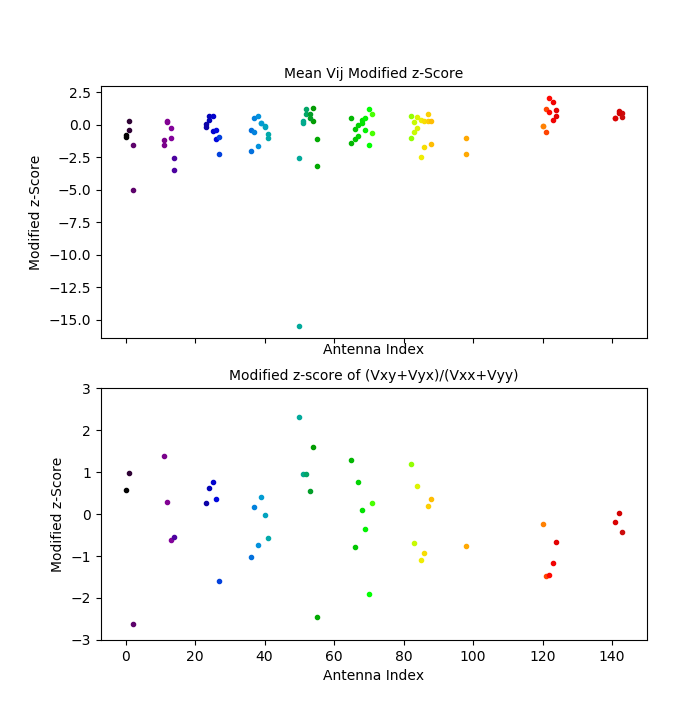
\includegraphics[width=0.7\textwidth]{chapters/data_processing/figures/metrics.png}
\caption[An example of the mean amplitude flagging metrics on exercised on HERA-47 data.]{An example of the mean amplitude flagging metrics on exercised on HERA-47 data. The top panel shows the mean amplitude flagging metric $M_i$, and the lower panel shows the cross-polarization metric $P_i$. The $E$ feed of antenna 50 shows at $\sim$15$\sigma$ deviation, causing it to be flagged from further processing.}
\label{fig:data_metrics}
\end{figure}

Figure~\ref{fig:data_metrics} shows the application of the metrics described above to raw HERA-47 data in the RTC system. Note that we plotted the modified \textit{z}-score and not
the raw metric. Traditionally the \textit{z}-score is defined as the deviation from the
mean divided by the standard deviation, and is a method to detect outliers.
However, since our metrics were not necessarily normally-distributed, we use the
modified \textit{z}-score defined as 

\begin{equation}\label{eqn:modifiedzscore}
    MZ_{i} = 0.6745\frac{|x_{i} - \tilde{x}|} {MAD},
\end{equation}

where $x_{i}$ is some data point (in our case this was a metric),
$\tilde{x}$ is the median of ${\{x_{i}\}}$, and MAD is the median absolute
deviation. \cite{Iglewicz.10} recommend that modified
\textit{z}-scores with an absolute value greater than 3.5 should be flagged as outliers.
In the analyses shown in Figure~\ref{fig:data_metrics}, we took the cut-off to be 5, to account for greater acceptable
variation in our metrics.

The top panel of figure \ref{fig:data_metrics} shows the modified \textit{z}-score for
the mean visibility metric as a function of antenna number.
Antenna 50E (East-West polarization) was a $\sim$15$\sigma$ outlier, indicating a problem
with amplification along the signal chain. Upon further inspection,
antenna 50E was shown to exhibit strange behavior, dropping in and out of the signal chain. Further
investigation is needed to know the root cause of this misbehavior. 

The bottom row of figure \ref{fig:data_metrics} shows the modified \textit{z}-score for the cross
polarization metric as a function of antenna number. There were no modified
\textit{z}-scores outside of the [-5,5] range, indicating that there were no cross polarized
antennas. Further inspection of the raw visibility data validated this finding.

\subsection{Flagging on {\tt omnical} $\chi^2$}

We developed a metric that identified days of PAPER-128 observations with poor overall {\tt omnical} $\chi^2$ values. Using the median of the $\chi^2$ values in the EoR band (channels 100--160; 150--180\,MHz), over all days of observation, we flagged days that exceeded the average of the median by one standard deviation from the mean. Figure~\ref{fig:data_chisq_flagging} shows an example of this flagging method used on the latter half of the first PAPER-128 observing season. Clearly, there were just a few JDs that had exceptionally high $\chi^2$ values. Our metric captures almost all of these outliers -- the possible exceptions being JDs 2456717 and 2456718.

\begin{figure}
\centering
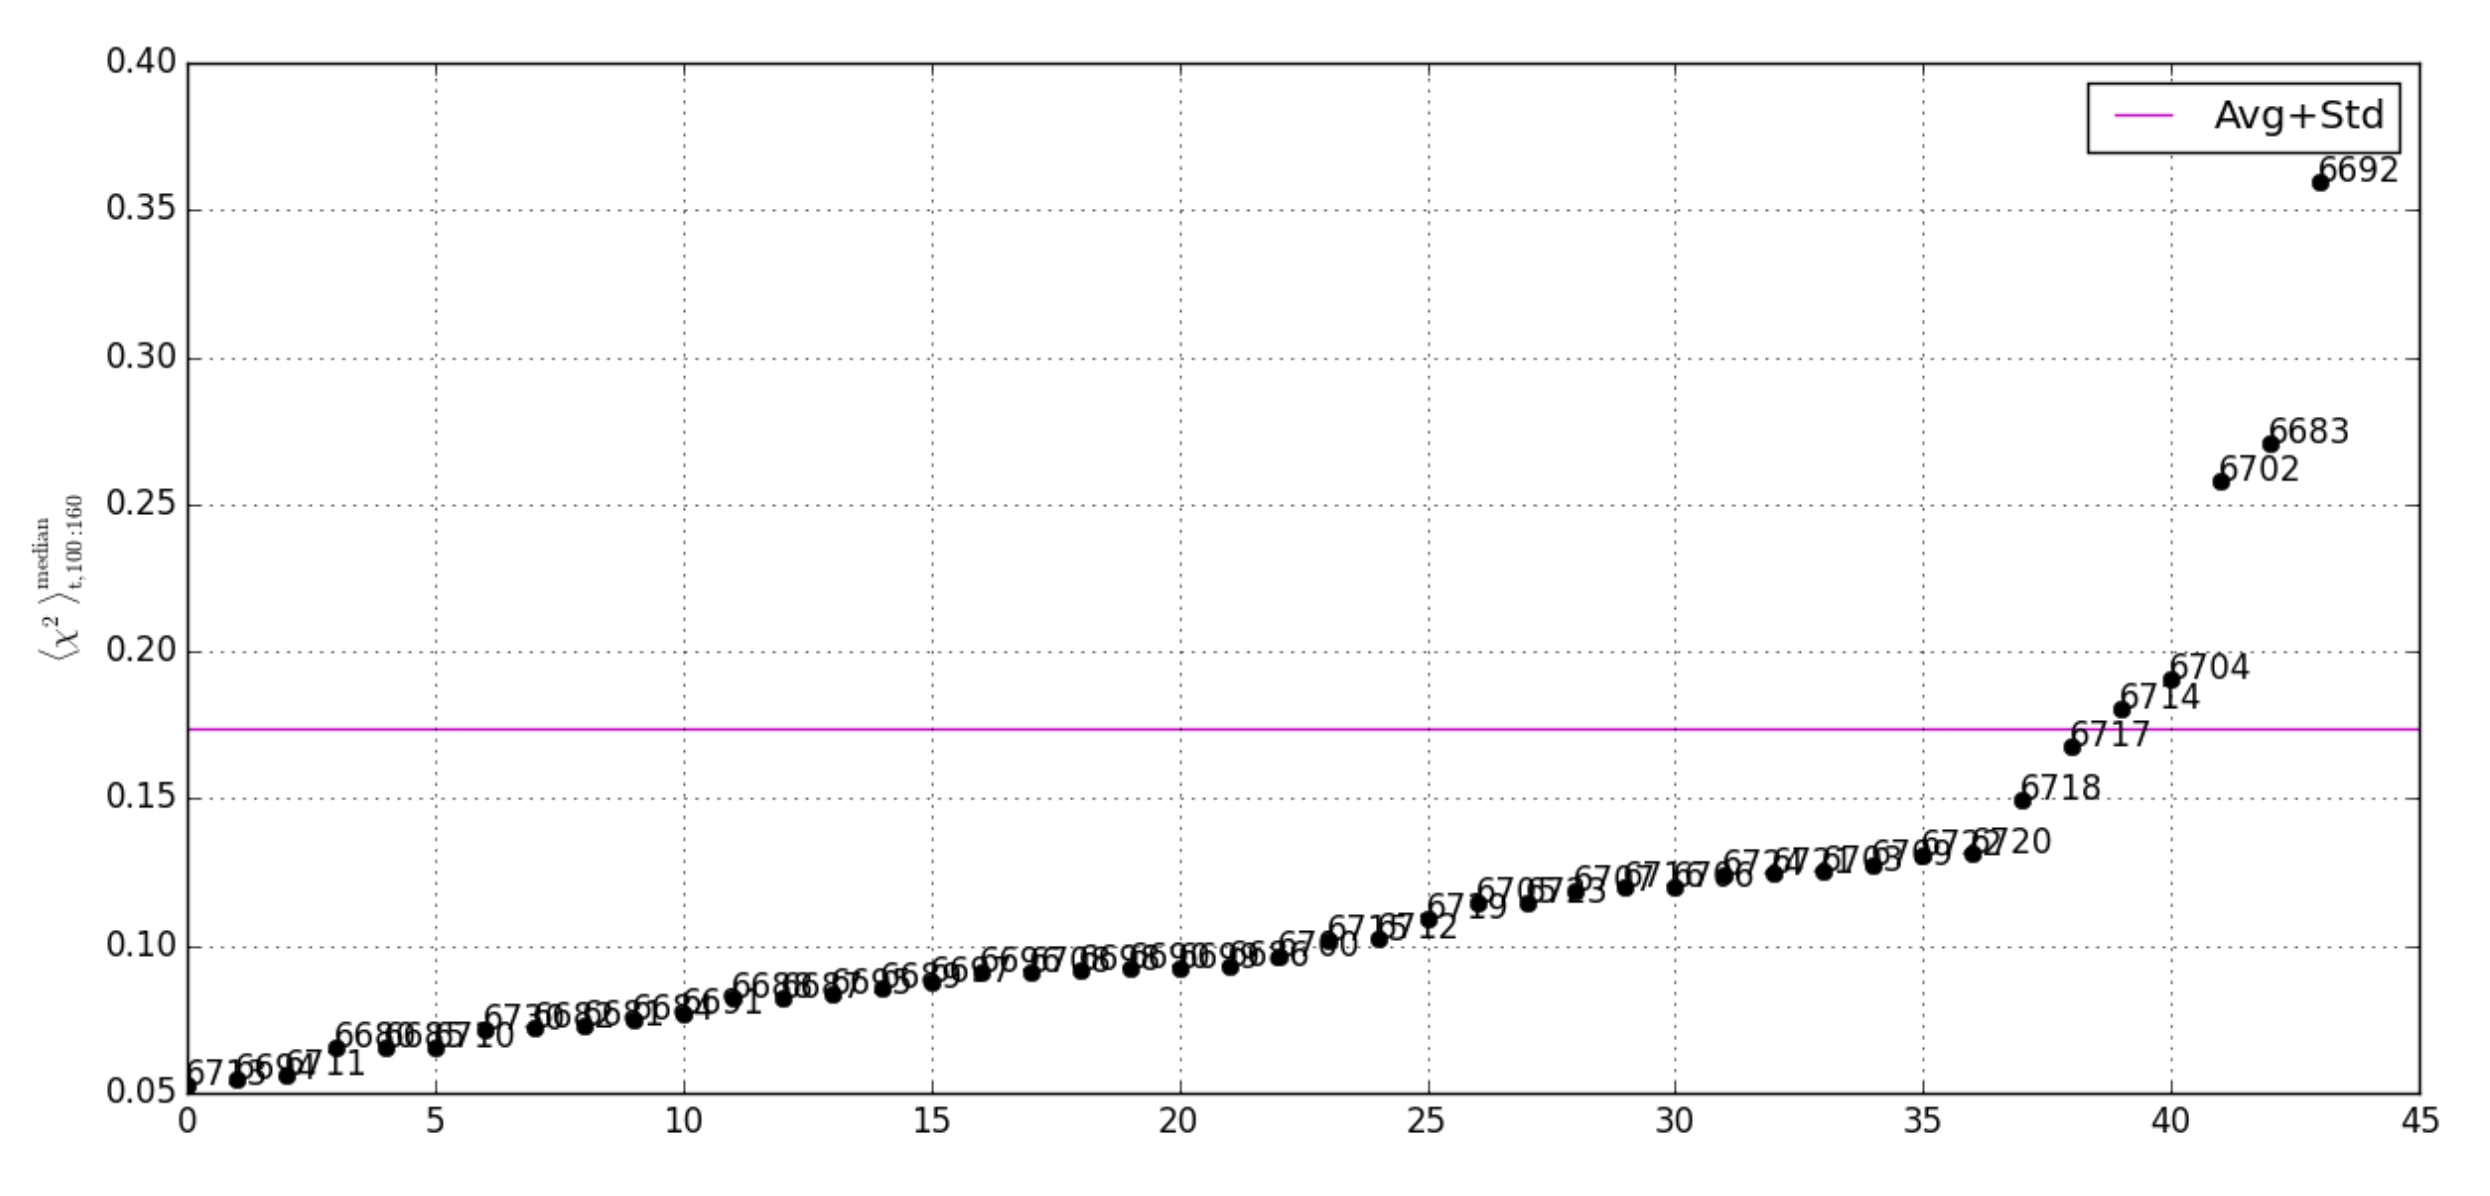
\includegraphics[width=0.7\textwidth]{chapters/data_processing/figures/chisq_flagging.png}
\caption[Flagging Julian Dates based on the median {\tt omnical} $\chi^2$ values in the 150--180\,MHz band.]{Flagging Julian Dates (JDs) based on the median {\tt omnical} $\chi^2$ values in the 150--180\,MHz band. Shown in pink is the flagging boundary. The JD labels have been abbreviated to drop the `245' prefix that they all share. Clearly, there are just a few JDs that have exceptionally high $\chi^2$ values.}
\label{fig:data_chisq_flagging}
\end{figure}

The {\tt omnical} software also provides $\chi^2_a$ values for each antenna $a$ -- that is, how much each antenna contributed to the overall non-redundancy of the array. The above sigma-clipping metric was applied to $\chi^2_a$, and was able to identify the same bad antennae using the mean amplitude flagging metric described in Equation~\ref{eq:meanvij}.
